\documentclass[fleqn]{article}
\usepackage[margin=1in]{geometry}
\usepackage{graphicx} % Required for inserting images
\usepackage{amsmath}
\usepackage{hyperref}
\usepackage{xparse}
\usepackage{tikz}
\usetikzlibrary{automata,positioning,decorations.text,topaths,arrows.meta,decorations.pathmorphing,quotes,calc}
\usetikzlibrary{backgrounds}
\usetikzlibrary{arrows,shapes}
\usetikzlibrary{tikzmark}
\tikzstyle{accepting}=[path picture={%
  \draw let 
    \p1 = (path picture bounding box.east),
    \p2 = (path picture bounding box.center)
    in
      (\p2) circle (\x1 - \x2 - 2pt);
  }]
\usetikzlibrary {automata,positioning,calc,shapes.geometric} 
% Pseudocode styling, thanks professor painter!
\usepackage[plain]{algorithm}
\usepackage{algorithmicx}
\usepackage{algpseudocode}
% allow input as a command for algorithms
\algnewcommand\algorithmicinput{\textbf{Input:}}
\algnewcommand\Input{\item[\algorithmicinput]}
% allow output as a command for algorithms
\algnewcommand\algorithmicoutput{\textbf{Output:}}
\algnewcommand\Output{\item[\algorithmicoutput]}
\algrenewcommand\textproc{\texttt}
\algnewcommand\algorithmicforeach{\textbf{foreach}}
\algdef{S}[FOR]{ForEach}[1]{\algorithmicforeach\ #1\ \algorithmicdo}

\usepackage{lmodern}
% \renewcommand*\familydefault{\sfdefault}
\newenvironment{lmodern}{\fontfamily{lmss}\selectfont}{\par}
% \algrenewcommand\ALG@beginalgorithmic{\begin{lmodern}}
% \algrenewcommand\ALG@endalgorithmic{\end{lmodern}}

\newif\ifanswerkey
\answerkeytrue

\NewDocumentEnvironment{answer}{ +b }{\ifanswerkey\newline \textbf{Solution:} #1\fi}{}

\title{CS/ECE374 Cramming Carnival Worksheet}
\author{}
\date{}

\begin{document}

\maketitle

\begin{center}
    This worksheet aims to ask problems similar to what you might see on the exam, but wasn't created with knowledge of exam content. Answers are available on the HKN website (\hyperlink{https://hkn.illinois.edu/services}{https://hkn.illinois.edu/services}).
\end{center}

\section{Regular Expressions}
Write a regular expression for the following languages:
\begin{enumerate}
    \item Strings that contain $01$ as a substring, but not $10$
    \begin{answer}
        Since $\Sigma = \{0,1\}$ and we can't have $10$, that means once we see a $1$, we can only see $1$s after it. So, our final expression is $\boxed{0^+ 1^+}$.
    \end{answer}
    \item Strings where every run of $1$s has odd length
    \begin{answer}
        We can represent a string containing \textit{only} an odd number of $1$s with the expression $1(11)^*$. We note that a string with an odd number of $1$s contains exactly one run of $1$s, so we can concatenate a bunch of these strings together with arbitrarily many $0$s in between to get our final answer: $\boxed{0^*(1(11)^*0^+)^*}$. Note that we must have at least one $0$ between each run so that the runs are separate.
    \end{answer}
    \item Strings that contain $101$ as a subsequence
    \begin{answer}
        A string $w$ has $101$ as a subsequence if we can write it as $w = x1y0z1w$ where
        $x,y,z,w \in \Sigma^*$, so we get $\boxed{(0+1)^* 1 (0+1)^* 0 (0+1)^* 1 (0 + 1)^*}$
    \end{answer}
    \item Strings representing a binary number divisible by $2$
    \begin{answer}
        A binary number is divisible by $2$ if it is even, i.e. the last digit is $0$.
        So, we allow any characters, followed by a $0$: $\boxed{(0+1)^* 0}$
    \end{answer}
    \item Strings representing a binary number that's a power of $2$
    \begin{answer}
        A binary string is a power of $2$ if it is of the form $10^n$ for $n \geq 0$. So, we want exactly one $1$ followed by zero or more $0$s: $\boxed{10^*}$
    \end{answer}
    \item Strings where runs of $1$s alternate between odd and even length (starting with odd length)
    \begin{answer}
        We already know the regex for an odd-length run is $1(11)^*$, and so the regex for an even-length run is $(11)^+$ (a run has nonzero length, so we use $+$ and not $*$). Now, we \textit{must} have at least one zero between the odd and even length runs, so one alternation (starting with even length) is given by the expression $(11)^+ 0^+ 1(11)^*$, and we want to repeat this arbitrarily many times, allowing for the string to begin with $0$s and have only one odd-length run: $\boxed{0^* 1(11)^* 0^+ ((11)^+ 0^+ 1(11)^* 0^+)^* + 0^*}$. We include the additional case of $0^*$ to handle when there are no runs of $1$s.
    \end{answer}
\end{enumerate}

\section{Short Answer}
Answer true or false for each question. Justify your answers.
\begin{enumerate}
    \item If $AB$ is not a context-free language, then at least one of $A$ and $B$ is not a CFL.
    \begin{answer}
        \boxed{True.} CFLs are closed under concatenation, so if $A$ and $B$ are both context-free, then so is $AB$.
    \end{answer}
    \item If $A$ is regular and $B$ is a CFL, then $AB$ may not be context free.
    \begin{answer}
        \boxed{False.} The concatenation of a regular language and a CFL is CFL.
    \end{answer}
    \item If $L$ is not regular, then $L^*$ is not regular.
    \begin{answer}
        \boxed{False.} Let $L = \{0^n 1^n : n \geq 0\} \cup \{0,1\}$. Since $0, 1 \in L$, $L^* = \{0, 1\}^*$ which is regular.
    \end{answer}
    \item When reading a string of length $n$, an NFA with $\epsilon$-transitions will be in at most $n+1$ different states.
    \begin{answer}
        \boxed{False.} The NFA may $\epsilon$ transition as much as it wants and thus may visit more than $n$ states. This claim is true for DFAs, though.
    \end{answer}
    \item A DFA recognizing strings with $101$ as a subsequence requires at least $2^3 = 8$ states.
    \begin{answer}
        \boxed{False.} $2^3 = 8$ states are required for $101$ as a sub\textit{string}, but not a sub\textit{sequence} - we can use only $4$ states which track what characters we've seen so far.
    \end{answer}
    \item For a regular language $L$, there exists an upper bound on the number of states required to represent $L$ as a DFA.
    \begin{answer}
        \boxed{False.} Myhill-Nerode (fooling sets) give us a \textit{lower bound}, but one can always add useless states to $Q$ so there is no upper bound.
        NOTE: this question is broken, ignore!!!!!!
    \end{answer}
\end{enumerate}

\section{Standalone NFAs and DFAs}
Provide an NFA or DFA that decides each language. Consider why you chose to use one representation over the other.
\begin{enumerate}
    \item $L = \{w \in \Sigma^* : \text{101 is a subsequence of}~w\}$
    \begin{answer}
        Since we're looking for a subsequence, we can ``greedily'' add more and more characters to the subsequence until we've seen the entire thing: \\
        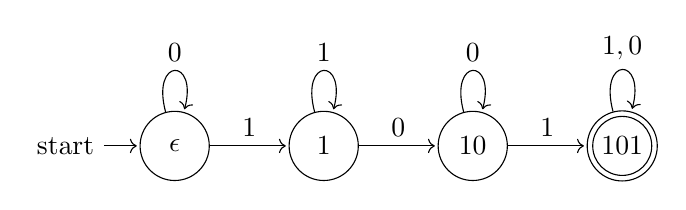
\begin{tikzpicture}[shorten >=1pt,node distance=1cm,auto]
    
          \node[state,initial]  (q_0)                      {$\epsilon$};
          \node[state]          (q_1) [right=of q_0] {$1$};
          \node[state]          (q_2) [right=of q_1] {$10$};
          \node[state,accepting](q_3) [right=of q_2] {$101$};
        
          \path[->] (q_0) edge node {$1$} (q_1)
                    (q_1) edge node {$0$} (q_2)
                    (q_2) edge node {$1$} (q_3)
                    (q_0) edge[loop above] node {$0$} (q_0)
                    (q_1) edge[loop above] node {$1$} (q_1)
                    (q_2) edge[loop above] node {$0$} (q_2)
                    (q_3) edge[loop above] node {$1,0$} (q_3);
        \end{tikzpicture} \\
        A DFA works fine here since we never have to make any choices and can always
        add a character to the subsequence as soon as we see it.
    \end{answer}
    \item $L = \{w \in \Sigma^* : \text{101 is a substring of}~w\}$
    \begin{answer}
        Since we're looking for a substring, we'll adapt the above DFA into an NFA that guesses when to start reading the substring (and since it's a substring, it shouldn't read any other characters between the $1$, $0$, or $1$): \\
        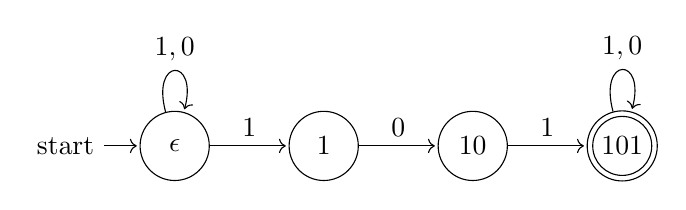
\begin{tikzpicture}[shorten >=1pt,node distance=1cm,auto]
    
          \node[state,initial]  (q_0)                      {$\epsilon$};
          \node[state]          (q_1) [right=of q_0] {$1$};
          \node[state]          (q_2) [right=of q_1] {$10$};
          \node[state,accepting](q_3) [right=of q_2] {$101$};
        
          \path[->] (q_0) edge node {$1$} (q_1)
                    (q_1) edge node {$0$} (q_2)
                    (q_2) edge node {$1$} (q_3)
                    (q_0) edge[loop above] node {$1, 0$} (q_0)
                    (q_3) edge[loop above] node {$1,0$} (q_3);
        \end{tikzpicture} \\
        Recall that as long as a correct guess exists, the NFA will take it, so this NFA accepts strings that have $101$ as a substring. Since we're missing some transitions here, we'll need to specify that missing transitions lead to a reject state.
    \end{answer}
    \item $L = \{w \in \{0,1,2\}^* : \sum_{i}w_i \equiv 0~(\text{mod}~5)\}$
    \begin{answer}
        We can't track the raw sum of all the digits in $w$, but since we can apply the modulus operator at every step of addition, we \textit{can} track the sum of the digits mod $5$ (which we want to be $0$ at the end). We don't want to make any guesses here, since every time we see a digit we just want to do addition.
        Formally, our DFA is written as 
        \[
            \begin{aligned}
                Q &= \{0,\dots,4\} \\
                s &= 0 \\
                A &= \{0\} \\
                \delta(q, i) &= (q + i) ~\text{mod}~ 5
            \end{aligned}
        \]
        which means that, at each new character, we update our current sum mod $5$ (stored in $q$) with the addition of the new digit, reapplying the mod to ensure we keep our output in $\{0,\dots, 4\}$.
    \end{answer}
    \item $L = \{w \in \Sigma^* : w = x111~\text{for some}~x \in \Sigma^*\}$
    \begin{answer}
        In simpler terms, the $L$ is the set of strings that end in $111$. We'll use the power of an NFA here to guess when our input string is about to end, and check for three $1$s. Since it's an NFA, it will guess at the correct time if our string does indeed end with three $1$s, and otherwise it will reject:
        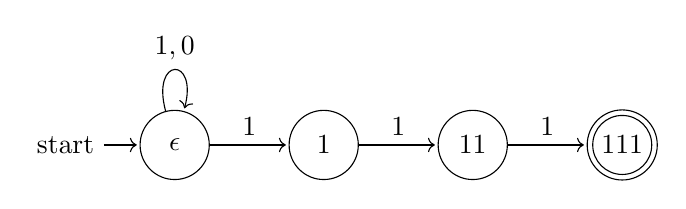
\begin{tikzpicture}[shorten >=1pt,node distance=1cm,auto]
    
          \node[state,initial]  (q_0)                      {$\epsilon$};
          \node[state]          (q_1) [right=of q_0] {$1$};
          \node[state]          (q_2) [right=of q_1] {$11$};
          \node[state,accepting](q_3) [right=of q_2] {$111$};
        
          \path[->] (q_0) edge node {$1$} (q_1)
                    (q_1) edge node {$1$} (q_2)
                    (q_2) edge node {$1$} (q_3)
                    (q_0) edge[loop above] node {$1, 0$} (q_0);
        \end{tikzpicture} \\
        Since we're missing some transitions here, we need to specify that these missing transitions lead to a reject state.
    \end{answer}
    \item $L_z = \{w \in \Sigma^* : z~\text{is a prefix of}~w\}$
    \begin{answer}
        We don't need any non-determinism here, since we don't need to guess where the start of our string is. Since all we know about $z$ is that it's an arbitrary string, we can write it as $z = z_1\cdots z_{|z|}$. We want the first character of an input string to be $z_1$, the second to be $z_2$, and so on. Since $z$ may have duplicate characters, we can't use $Q = \{z_1,\dots z_{|z|}\}$ but we can use $Q = \{1, \dots, |z|\}$. These states will allow us to track how much of $z$ we've read from our input (we can move from $i$ to $i+1$ if we see $z_{i+1}$, and reject otherwise), so we'll need one additional state for when we've seen nothing, giving us a final answer of:
        \[
            \begin{aligned}
                Q &= \{0,\dots,|z|\} \\
                s &= 0 \\
                A &= \{|z| + 1\} \\
                \delta(i, z_{i+1}) &= i + 1 ~\text{for } i < |z| \\
                \delta(|z|, x) &= |z| ~\forall x
            \end{aligned}
        \]
        This definition only includes transitions of the form $i \to i+1$ when the character $z_{i+1}$ is seen, so we'll need to add the magic sentence that ``any missing transitions lead to a reject state.'' If this answer is a bit confusing, don't worry - fully generic solutions can be that way. Drawing out the DFA described above for a concrete $z$ (try $101$) might make things more clear.
    \end{answer}
\end{enumerate}

\section{Product Construction}
Let $L_1, L_2, L_3$ be regular languages. Provide an NFA or DFA that decides each language. Your final answer should use tuple notation, and not be a drawing.
\begin{enumerate}
    \item $L_{eo} = \{w \in \Sigma^* : \#(1,w) \equiv \#(0, w) \equiv 1~(\text{mod}~2)\}$
    \begin{answer}
        When we see a language like  this with a multipart condition, it's helpful to break it down into smaller languages. In particular, let
        $L_0 = \{w \in \Sigma^* : \#(0, w)~\text{is odd}\}$ and $L_1 = \{w \in \Sigma^* : \#(1, w)~\text{is odd}\}$. We can see that $L_{eo} = L_1 \cap L_2$. So, let's first create machines for $L_0$: \\
        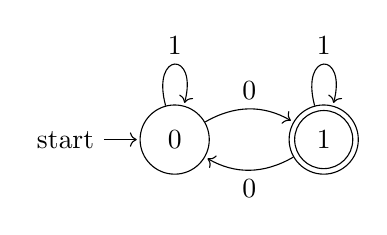
\begin{tikzpicture}[shorten >=1pt,node distance=1cm,auto]
    
          \node[state,initial]   (q_0)                      {$0$};
          \node[state, accepting](q_1) [right=of q_0] {$1$};
        
          \path[->] (q_0) edge[bend left] node {$0$} (q_1)
                    (q_1) edge[bend left] node {$0$} (q_0)
                    (q_0) edge[loop above] node {$1$} (q_0)
                    (q_1) edge[loop above] node {$1$} (q_1);
        \end{tikzpicture} \\
        and for $L_1$: \\
        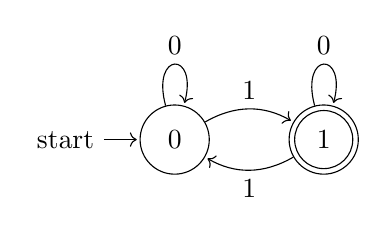
\begin{tikzpicture}[shorten >=1pt,node distance=1cm,auto]
    
          \node[state,initial]   (q_0)                      {$0$};
          \node[state, accepting](q_1) [right=of q_0] {$1$};
        
          \path[->] (q_0) edge[bend left] node {$1$} (q_1)
                    (q_1) edge[bend left] node {$1$} (q_0)
                    (q_0) edge[loop above] node {$0$} (q_0)
                    (q_1) edge[loop above] node {$0$} (q_1);
        \end{tikzpicture} \\
        We'll call these machines $M_0$ and $M_1$. Now, we can set up scaffolding to run $M_0$ and $M_1$ in parallel:
        \[
            \begin{aligned}
                Q &= Q_0 \times Q_1 \\
                s &= (s_0, s_1) \\
                \delta((q_0,q_1), x) &= (\delta_0(q_0,x),\delta_1(q_1,x))
            \end{aligned}
        \]
        Now, we want to accept an input string if it is accepted by both $M_0$ and $M_1$, meaning our simulation ends in a state of the form $(a_0, a_1)$ where $a_0 \in A_0$ and $a_1 \in A_1$. This is precisely the set of states defined by $A_0 \times A_1$ so we get
        \[
            A = A_0 \times A_1
        \]
    \end{answer}
    \item $L = \{w : w \in \overline{L_1 \cup L_2}\}$
    \begin{answer}
        Once again, let's set up the scaffolding to run $M_1$ and $M_2$ in parallel:
        \[
            \begin{aligned}
                Q &= Q_1 \times Q_2 \\
                s &= (s_1, s_2) \\
                \delta((q_1,q_2),x) &= (\delta_1(q_1,x), \delta_2(q_2,x))
            \end{aligned}
        \]
        We want to accept an input string $w$ if it is in $\overline{L_1 \cup L_2}$. By DeMorgan's law, this means we want to accept $w$ if it is not in $L_1$ \text{and} it is not in $L_2$; that is, we accept $w$ if both $M_1$ and $M_2$ reject it. $M_1$ and $M_2$ reject $w$ when they end in a state which is not an accepting state (that is, a state in the set $Q_i \setminus A_i$, so we can require both machines to end in such a state with a cartesian product:
        \[
            A = (Q_1 \setminus A_1) \times (Q_2 \setminus A_2)
        \]
    \end{answer}
    \item $L = \{w : w~\text{is in at least two of}~L_1,L_2,L_3\}$
    \begin{answer}
        Since $L_1,L_2,L_3$ are regular, we can assume that we have DFAs $M_1,M_2,M_3$ that decide each language. Now, we want to build a machine $M$ that simulates running $M_1, M_2, M_3$ on an input string $w$, and based on the end states of $M_1,M_2,M_3$ will decide whether to accept or reject $w$. Let's first set up the scaffolding to simulate running these machines:
        \[
            \begin{aligned}
                Q &= Q_1 \times Q_2 \times Q_3 \\
                s &= (s_1, s_2, s_3) \\
                \delta((q_1,q_2,q_3),x) &= (\delta_1(q_1,x), \delta_2(q_2,x), \delta_3(q_3,x))
            \end{aligned}
        \]
        Now we need to figure out $A$. $w \in L_i$ if running $w$ through $M_i$ ends in an accept state. Since we are simulating each machine with the product construction, that means $w \in L_i$ if we end in a state $(\dots,q_i,\dots)$ where $q_i \in A_i$. For example, $w \in L_1$ if we end in a state where the first element is one of the accept states of $M_1$. Using this idea, we can think of all the cases where our state represents acceptance by at least two machines, and combine them all:
        \[
            \begin{aligned}
                A &= A_1 \times A_2 \times Q_3 &\text{(accepted by }M_1\text{ and }M_2\text{ and maybe }M_3\text{)} \\
                &~~~\cup A_1 \times Q_2 \times A_3 &\text{(accepted by }M_1\text{ and }M_3\text{ and maybe }M_2\text{)} \\
                &~~~\cup Q_1 \times A_2 \times A_3 &\text{(accepted by }M_2\text{ and }M_3\text{ and maybe }M_1\text{)}
            \end{aligned}
        \]
    \end{answer}
    \item $L = \{w : w~\text{has an odd number of}~1\text{s and contains the subsequence}~101\}$
    \begin{answer}
        We can write this as the intersection of two languages: the set of strings with an odd number of $1$s, and the set of strings containing the subsequence $101$. Even better, earlier in this worksheet, we've created machines for each of these languages! Call the machines $M_{1s}$ and $M_{101}$. We want to run these machines in parallel, so we'll once again set that up:
        \[
            \begin{aligned}
                Q &= Q_{1s} \times Q_{101} \\
                s &= (s_{1s}, s_{101}) \\
                \delta((q_{1s}, q_{101}), x) &= (\delta_{1s}(q_{1s}), \delta_{101}(q_{101},x))
            \end{aligned}
        \]
        Now, we want to accept a string if both $M_{1s}$ and $M_{101}$ accept it. As before, this means we have
        \[
            A = A_{1s} \times A_{101}
        \]
    \end{answer}
    \item $L_{ps} = \{w : w~\text{ends in}~111\wedge ~\text{the digits in $w$ sum to a number not divisible by}~5\}$
    \begin{answer}
        This looks complex, but we can break it down into smaller languages. Let $L_1$ be the set of strings that end in $111$, and $L_2$ be the set of strings whose digits sum to a number divisible by $5$. We can thus rewrite $L_{ps} = L_1 \cap \overline{L_2}$. Now, we can run both machines (call them $M_1$ and $M_2$) in parallel as normal:
        \[
            \begin{aligned}
                Q &= Q_1 \times Q_2 \\
                s &= (s_1, s_2) \\
                \delta((q_1,q_2), x) &= (\delta_1(q_1,x),\delta_2(q_2,x))
            \end{aligned}
        \]
        We want to accept an input string when $M_1$ accepts it and $M_2$ rejects it, so that means we want to end in a state of the form $(a_1,r_2)$ where $a_1 \in A_1$ and $r_2 \in Q_2 \setminus A_2$. This is precisely the elements of the set $A_1 \times (Q_2 \setminus A_2)$ so we have
        \[
            A = A_1 \times (Q_2 \setminus A_2)
        \]
    \end{answer}
\end{enumerate}

\section{Language Transformations}
Prove that each of the following languages are regular by creating an NFA, DFA, or regular expression for them.
\begin{enumerate}
    \item Let $\Sigma = \{0,1,2\}$ and let $\text{replace}(w)$ replace every $1$
    in $w$ with a $2$ (ex $\text{replace}(120) = 220$). Define $\text{Two}(L) = \{\text{replace}(w) : w \in L\}$.
    \begin{answer}
        Here, we want to go from a string to which $\text{replace}$ has been applied to the original string. This means that our NFA $M'$ for $\text{Two}(L)$ should simulate a DFA $M$ for $L$, and when it sees a $2$, it should choose to control the simulation by either (a) leaving the $2$ (i.e. it was a $2$ in the original string) or (b) turning it into a $1$ (i.e. it was a $1$ in the original string). We don't need to store any extra information, so we can use
        \[
            \begin{aligned}
                Q' &= Q \\
                A' &= A \\
                s' &= s \\
                \delta'(q, x) &= \begin{cases}
                    \{\delta(q,x)\} & x \neq 2 \\
                    \{\underbrace{\delta(q,1)}_{\text{this $2$ was a $1$ before}},\underbrace{\delta(q,2)}_{\text{this $2$ was a $2$ before}}\} & x = 2
                \end{cases}
            \end{aligned}
        \]
        Since an NFA always makes the correct guess (if one exists), giving it the power to make both guesses ensures it will accept strings if they are the result of transforming a string in $L$.
    \end{answer}
    \item Using $\text{replace}$ as above, define $\text{UnTwo}(L) = \{w \in \Sigma^*: \text{replace}(w) \in L\}$
    \begin{answer}
        Here, we want to go in the reverse direction, and apply $\text{replace}$ to our input string as we feed it into $M$. This means every time we see a $1$, we send a $2$ to $M$, and keep everything else the same:
        \[
            \begin{aligned}
                Q' &= Q \\
                A' &= A \\
                s' &= s \\
                \delta(q,a) &= \begin{cases}
                    \delta(q,2) & a = 1 \\
                    \delta(q,a) & \text{o.w.}
                \end{cases}
            \end{aligned}
        \]
    \end{answer}
    \item Let $\text{prepend}(w)$ prepend $11$ to $w$ (ex $\text{prepend}(10) = 1110$). Define $\text{Prepend}(L) = \{\text{prepend}(w) : w \in L\}$.
    \begin{answer}
        A string in $\text{Prepend}(L)$ has two $1$s and then a string in $L$, so we want to build a DFA that will ``eat'' those $1$s, and then start simulating $M$ on its input:
        \[
            \begin{aligned}
                Q' &= Q \cup \{0, 1\} \\
                s' &= 0 \\
                A' &= A \\
                \delta'(0, 1) &= 1 \\
                \delta'(1, 1) &= s \\
                \delta'(q, x) &= \delta(q, x)
            \end{aligned}
        \]
        We haven't defined all transitions from states $0$ and $1$ so we'll assume they go to a reject state.

        There's a more clever solution to this though. You might notice that the machine we constructed above looks like a special case of concatenating two machines together. Concatenation is easier with regular expressions, though, and since $L$ is regular that means we have some regular expression $r_L$ for it. The expression $r = 11r_L$ thus decides $\text{Prepend}(L)$.
    \end{answer}
    \item Let $\text{add}(w)$ append $111$ to $w$ (ex $\text{add}(10) = 10111$). Define $\text{Add}(L) = \{\text{add}(w) : w \in L\}$.
    \begin{answer}
        We want to take a string of the form $x111$, and check that $x$ is in $L$. Using the idea of the standalone NFA/DFAs question on checking for a suffix of $111$, we want our NFA $M'$ for $\text{Add}(L)$ to simulate running $M$ on an input until it guesses that $M$ is done and it's time to read $111$. We don't want to just arbitrarily check for $111$ though - we only want to do so after reading a string $x$ that $M$ \textit{accepts} - this means that from every accept state in $M$, we want to allow our NFA to choose that $x$ has been read and that it's time to begin reading $101$. This is exactly what an $\epsilon$ transition allows us to do, so we want to build something like this: \\
        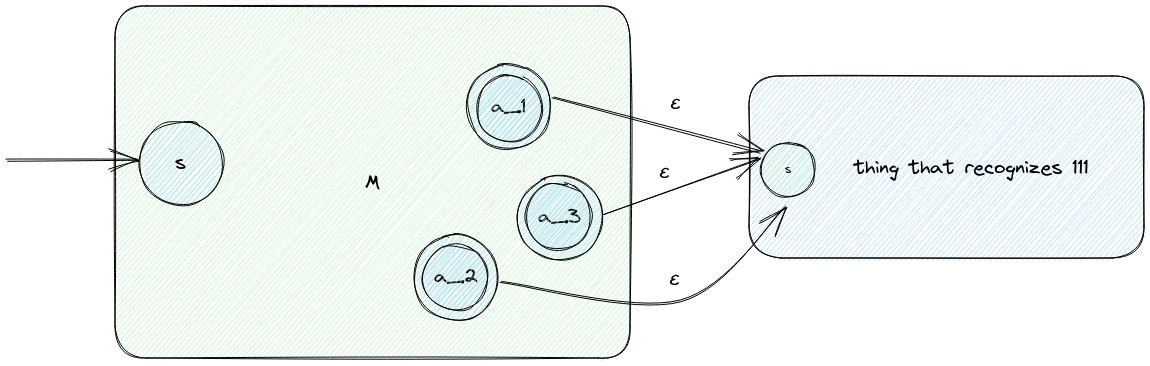
\includegraphics[width=6.25in]{figures/add_nfa.png}
        We can formally encode this as follows:
        \[
            \begin{aligned}
                Q' &= Q \cup \{\epsilon, 1, 11, 111\} \\
                A' &= \{111\} \\
                s' &= s \\
                \delta'(q,x) &= \{\delta(q,x)\} \\
                \delta'(q,\epsilon) &= \begin{cases}
                    \emptyset & q \notin A \\
                    \{\epsilon\} & q \in A
                \end{cases}
            \end{aligned}
        \]
        We have to change the accept state here because we must enforce that we transition from $M$ to the $111$ suffix.

        As with the previous question, there's a more clever solution. Can you spot it? All we're doing is concatenating the language $\{111\}$ after $L$, so we can create the following regular expression which decides $\text{Add}(L)$: $r = r_L 111$.
    \end{answer}
    \item Let $\text{d2}(w)$ delete the second-to-last character of $w$ (ex $\text{d2}(1010) = 100$). Define $\text{D2}(L) = \{\text{d2}(w) : w \in L\}$.
    \begin{answer}
        We want to take a string to which $\text{d2}$ has been applied and check if the original string is in $L$. Since there's two possibilities for the character that could've been deleted, $0$ or $1$, we'll use the power of an NFA to guess (correctly) which character to insert. We also need to use non-determinism to guess \textit{when} to insert the second-to-last character: after we insert it, we should see only one more character. We'll need additional state to track this, which we can handle with a product:
        \[
            \begin{aligned}
                Q' &= Q \times \{n,y,d\} \\
                s' &= (s, 0) \\
                \delta'((q, n), x) &= \{(\delta(q,x), n)\} \\
                \delta'((q, y), x) &= \{(\delta(q,x), d\} \\
                \delta'((q, n), \epsilon) &= \{(\delta(q, 1), y), (\delta(q,0), y)\}
            \end{aligned}
        \]
        A state of the form $(q,n)$ means the machine $M$ for $L$ is in state $q$ and we have not inserted the second-to-last character; $(q,y)$ means we just inserted the second-to-last character, and $(q,d)$ means we should be done reading the string. Since there are no outgoing transitions from any $(q,d)$ state, any early guesses are automatically invalid. We use the $\epsilon$-transition to allow the NFA to insert a single digit into the input string, since the $\epsilon$-transition goes from $(q,n)$ to $(q',y)$ only one such insert may occur. Now what should $A$ be? We want to accept states of the form $(a,d)$, meaning we reached an accept state in $M$ and inserted a $1$ or $0$ at the right position. This is precisely the set of states given by
        \[
            A' = A \times \{d\}
        \]
    \end{answer}
    \item Using $\text{d2}$ as above, define $\text{A2}(L) = \{w : \text{d2}(w) \in L\}$.
    \begin{answer}
        We want to go in reverse of what we just did, and our NFA $M'$ should skip sending the second-to-last character into the DFA $M$ for $L$. In other words, at some point, we want to choose to skip the current character, and after that point, we should only see one more character (meaning the character we deleted was the second-to-last). Once again, we'll need a product construction to track this:
        \[
            \begin{aligned}
                Q' &= Q \times \{n, y, d\} \\
                s' &= (s, n) \\
                \delta'((q, n), x) &= \{\underbrace{(\delta(q,x), n)}_{\text{don't skip}}, \underbrace{(q, y)}_{skip}\} \\
                \delta'((q,y), x) &= \{(\delta(q,x), d)\}
            \end{aligned}
        \]
        A state $(q,n)$ means $M$ is in state $q$ and we haven't skipped a character yet, from this state we can transition to $(q,y)$ which represents $M$ is in state $q$ and we've skipped what might be the second-to-last character; after reading the last character we end up in $(q',d)$ which indicates we are done, there are no outgoing transitions from here, so if we made a bad guess, $M'$ would reject. We want to accept when we got to a valid string in $L$ (i.e. the first element is in $A$) and after we deleted the second-to-last character and finished reading the input, so once again, we get
        \[
            A' = A \times \{d\}
        \]
    \end{answer}
    \item Let $\text{insert0}(w)$ be a function that generates all the ways to insert a single $0$ into $w$ at an arbitrary location (ex $\text{insert0}(10) = \{010, 100\}$). Define $\text{AddZero}(L) = \cup_{w \in L}\text{insert0}(w)$.
    \begin{answer}
        This one looks a little harder because $\text{insert0}$ returns a set, not a single string. But, if we think about a string in $\text{insert0}(w)$, it's just $w$ but with a $0$ inserted at some location; so, to check if a string $w'$ is in $\text{AddZero}(L)$, we want to see if we can remove some $0$ from that string and get a string $w \in L$. We'll use the power of an NFA to guess which $0$ to remove, meaning when we see a $0$, we should have two transitions: feed the $0$ into $M$, or simply ignore it. If we ignore it, we want to record that we've done our one and only permissible deletion, so we'll need a product construction:
        \[
            \begin{aligned}
                Q' &= Q \times {F, T} \\
                s' &= (s, F) \\
                \delta'((q, T), x) &= \{(\delta(q,x), T)\} \\
                \delta'((q, F), x) &= \{\underbrace{(\delta(q,x), F)}_{\text{don't skip}}, \underbrace{(q, T)}_{\text{skip and record}}\}
            \end{aligned}
        \]
        Since we \textit{must} perform exactly one zero removal to get back to $L$, our accepting states are given by
        \[
            A' = A \times \{T\}
        \]
    \end{answer}
    \item Using $\text{insert0}$ as above, define $\text{DeleteZero}(L) = \{w \in \Sigma^* : \text{insert0}(w) \cap L \neq \emptyset\}$
    \begin{answer}
        First we'll begin by deciphering the notation here: the condition on the set says that a string $w$ is in $\text{DeleteZero}(L)$ if at least one of the ways to insert a $0$ into the string results in a string in $L$. So, to check this condition, we want to build a machine $M'$ that guesses the correct location to insert a single $0$ into an input string $w$ as it feeds the string into a DFA $M$ for $L$. Since we want to do exactly one insertion, we'll need a product construction similar to the previous question:
        \[
            \begin{aligned}
                Q' &= Q \times \{F, T\} \\
                s' &= (s, F) \\
                \delta'((q,B), x) &= \{(\delta(q,x),B)\} \\
                \delta'((q,F), \epsilon) &= \{(\delta(q, 0), T)\}
            \end{aligned}
        \]
        Similar to before, we only want to accept after we've modified the input string, so we'll set
        \[
            A' = A \times \{T\}
        \]
    \end{answer}
\end{enumerate}

\section{Fooling Sets}
Find the largest fooling set you can for each of the given languages.
\begin{enumerate}
    \item $L = \{0^n w 1^n : w \in \Sigma^* \wedge |w| \leq 3 \wedge n \geq 0\}$
    \begin{answer}
        Remember that for $L' = \{0^n 1^n : n \geq 0\}$ we used the fooling set $F' = \{0^n : n \geq 0\}$: we can do something similar here. The tricky part is $w$: consider two strings from $F'$, say $0$ and $00$: if I use a suffix of $11$, both strings are in $L$ because $w = 1$ for the first string, and $w = \epsilon$ for the second. To get around this, we'll control the value of $w$ ourselves by providing three additional $1$s after each string in our fooling set, so 
        $\boxed{F = \{0^n 111 : n \geq 0\}}$. Now, let's show that this fooling set works. Consider strings $x = 0^i 111$ and $y = 0^j 111$ from $F$, and assume $i > j$. Now, choose $z = 1^i$: clearly, $xz \in L$, but $yz \notin L$, since $yz = 0^j 111 1^i$: since $i > j$, we can rewrite $yz = 0^j 111 (1^{i-j}) (1^j)$ but since $i - j > 0$, $|111 ^{i-j} > 3$, which is the maximum length for the middle string $w$.

        It's worth noting that the first time I tried to write this solution, I didn't make any assumptions about $i > j$, and got stuck, because if $j < i$ then there are some edge cases where suffix $z$ does not work. Since you can always assume that either $i > j$ or $i < j$, it's worth just making this choice at the start of each fooling set proof so you can use it if necessary.
    \end{answer}
    \item $L = \{0^n w 1^n : w \in \Sigma^* \wedge n \geq 0\}$
    \begin{answer}
        Since we can choose $n = 0$ and let $w$ be anything, $L = \Sigma^*$. Since this set contains all strings over $\Sigma$, we can't create a fooling set with more than one element, because there's no distinguishing suffixes to choose (since appending any suffix still results in a string in $\Sigma^*$). So, the biggest fooling set we can create has exactly one element. We can pick $\boxed{F = \{0\}}$. The size of this set is also the minimum number of states required to create a DFA for $L$. Can you think of a one state DFA for this language?
    \end{answer}
    \item $L = \{0^n 1^m : n~\text{is divisible by}~m \wedge n,m \geq 0\}$
    \begin{answer}
        There's two solutions to this problem. We'll present the ``slick'' one first, and then the more traditional one. Recall that $n$ is not divisible by $m$ if $m > n$, and that $n$ is divisible by itself. Recall from the previous problem that we can also choose which string picked from our fooling set is shorter. Let $\boxed{F = \{0^n : n \geq 1\}}$. Consider $x = 0^i$ and $y = 0^j$ where $i > j$. Let $z = 1^i$. Since $i$ is divisible by $i$, $xz \in L$, but since $i > j$, $j$ is not divisible by $i$, and $yz \notin L$, so $F$ is a fooling set. Note that we chose $n \geq 1$ as our condition here because it removes division by $0$ edge cases.

        A more traditional solution to this problem is to remember that no two primes are divisible by one another, and create a fooling set containing strings of the form $0^i$ for prime $i$. The same suffix as above works, since a prime is always divisible by itself and no other primes. In general, when you see divisibility conditions but on modular arithmetic, messing around with primes can be useful.
    \end{answer}
    \item $L = \{z0z^r : z \in \Sigma^*\}$
    \begin{answer}
        If $z$ ends in a $0$ (or contains a $0$ for that matter), it might be tedious to show that a distinguishing suffix for our fooling set is in fact a distinguishing suffix. Intuitively, $L$ is not regular because a DFA would have to store all of $z$. Let's exploit that by making a fooling set containing all of the $z$s (not containing any $0$s) that a DFA would have to store: $\boxed{F = \{1^n : n \geq 1\}}$. Now, consider two strings from $F$, $x = 1^i$ and $y = 0^j$:  let $z = 01^i$: since $1^i = (1^i)^R$, then $xz \in L$ but $yz \notin L$ since $1^j \neq (1^i)^R$. The strategy we used to build $F$ here is a common one: when there are things in the middle, we want to try our best to control exactly where they show up in strings we pull from the fooling set, since this makes the proof easier.
    \end{answer}
    \item (Hard.) $L_k = \{w : \text{the}~ k\text{th to last character of}~w~\text{is } 1\}$
    \begin{answer}
        Intuitively, we want to make a fooling set so that our distinguishing suffix $z$ controls whether the $k$th-to-last character is $1$. Since the distinguishing suffix $z$ must be the same for any two strings $x$ and $y$, this means that $x$ and $y$ must, at the very least, have a difference in one of their last $k$ digits. The only way we can ensure this is with a fooling set of $\boxed{F = \{w \in \Sigma^* : |w| = k\}}$. Now, let's fix two elements $x$ and $y$ in $F$. We know that $x \neq y$, so there is some character where $x$ and $y$ differ. Thus, we can write $x = \alpha 1 \beta$ and $y = \alpha 1 \gamma$. Now, if $|\gamma| = k-1$, we can pick $z = \epsilon$ and we're done, since the $k$th-to-last character already differs in $x$ and $y$. Otherwise, since $|x| = |y| = k$, we have $|\gamma| = |\beta| < k$, so we can let $z = 1^{k - |\gamma|}$, which will place the $1$ and $0$ in the $k$th-to-last position of $x$ and $y$, respectively, resulting in $xz \in L$ and $yz \notin L$.

        The trick we used here of focusing on a single character difference between two strings is a useful technique to keep in mind for fooling set problems.
    \end{answer}
\end{enumerate}

\section{Context Free Languages}
Write a context-free grammar for each of the provided languages.
\begin{enumerate}
    \item $L = \{1^n 0^{3n} : n \geq 0\}$
    \begin{answer}
        We can build such strings outside-in, adding one $1$ and three $0$s at a time:
        \[
            \boxed{S \to \epsilon ~|~ 1S000}
        \]
    \end{answer}
    \item $L = \{w \in \Sigma^* : w~\text{has exactly two more }1\text{s than }0\text{s}\}$
    \begin{answer}
        We'll solve this problem by first creating a CFG that enforces that the number of $1$s and $0$s remains the same:
        \[
            S \to \epsilon~|~ 0S1~|~ 1S0
        \]
        We can modify this to require exactly one more $1$ than $0$ by changing to
        \[
            S \to 1 ~|~ 0S1 ~|~ 1S0
        \]
        Now we need this twice:
        \[
            \begin{aligned}
                S &\to AA \\
                A &\to 1 ~|~ 0A1 ~|~ 1A0
            \end{aligned}
        \]
    \end{answer}
    \item $L = \{w 0^n 1^n w^r : w \in \Sigma^* \wedge n \geq 0\}$
    \begin{answer}
        We can use the same idea as the previous problem and build a CFG in two phases: writing a palindrome, and then writing $0^n 1^n$. We can generate $w w^R$ by the following CFG:
        \[
            \begin{aligned}
                S &\to \epsilon ~|~ 1 S 1 ~|~ 0 S 0
            \end{aligned}
        \]
        Since we're going outside-in, what remains is to fill in the middle with $0^n 1^n$ for $n \geq 0$, which you may remember we can generate with the following CFG:
        \[
            S \to 0S1 ~|~ \epsilon 
        \]
        Combining these together, we get
        \[
            \boxed{
            \begin{aligned}
                S &\to S_1 ~|~ 1 S 1 ~|~ 0 S 0 \\
                S_1 &\to 0S1 ~|~ \epsilon
            \end{aligned}}
        \]
    \end{answer}
\end{enumerate}

\noindent Describe the languages generated by each context-free grammar.
\begin{enumerate}
    \item 
    \[
        \begin{aligned}
            S \to 00 S 1~|~ \epsilon
        \end{aligned}
    \]
    \begin{answer}
        Here, we keep adding two more $0$s than $1$s until reaching a base case of empty string,
        so $\boxed{L = \{0^{2n} 1^{n} : n \geq 0\}}$
    \end{answer}
    \item 
    \[
        \begin{aligned}
            S &\to 2 S 3~|~ 3 S 2 ~|~ R \\
            R &\to 11R ~|~ R00 ~|~ \epsilon
        \end{aligned}
    \]
    \begin{answer}
        First, we'll begin by deciphering $R$: starting from $\epsilon$, we can build $11R$, then $1111R$, and so on, and any time we insert a $00$, the $00$ goes to the right of the $R$:
        $11R00$, $11R0000$, and so on. So, this generates $L_r = \{(11)^{i} (00)^{j} : i,j \geq 0\}$.
        This is only generated after $S$ finishes, and $S$ generates outer strings with the same number of $2$s and $3$s. So, we have\\$\boxed{L = \{w (11)^{i} (00)^{j} z : \#(2,wz) = \#(3,wz) \wedge i,j \geq 0 \wedge |w| = |z|\}}$.
    \end{answer}
    \item
    \[
        \begin{aligned}
            S &\to 0 S 1 | 1 S 0 | 1 | 0
        \end{aligned}
    \]
    \begin{answer}
        We observe that the grammar continuously adds $1$s and $0$s in equal number until stopping by either adding a single $1$ or single $0$, so the end result is a string with exactly one more $1$ than $0$s, or vice versa. $\boxed{L = \{w : |\#(0,w) - \#(1,w)| = 1\}}$
    \end{answer}
\end{enumerate}

\section{Sums and Recurrences}
Provide a tight asymptotic upper bound for each of the following sums and recurrences.
\begin{enumerate}
    \item $\sum^n_{i=1} i \sqrt{i}$
    \begin{answer}
        $O(n^{\frac{5}{2}})$. \\
        \text {Lower bound}
        \[
            \sum^{n}_{i=1} i\sqrt{i}
            = \sum^{n}_{i=1} i^{\frac{3}{2}} 
            \geq \sum^n_{i=\frac{n}{2}} i^{\frac{3}{2}}
            \geq \sum^n_{i=\frac{n}{2}} \left(\frac{n}{2}\right)^{\frac{3}{2}}
            = \frac{n}{2} \left(\frac{n}{2}\right)^{\frac{3}{2}}
            = (\frac{n}{2})^{\frac{5}{2}}
        \]
        \text {Upper bound}
        \[
            \sum^{n}_{i=1} i\sqrt{i}
            \leq \sum^{n}_{i=1} n\sqrt{n}
            = n^{\frac{5}{2}}
        \]
        Therefore tight asymptotic bound is $O(n^{\frac{5}{2}})$
    \end{answer}
    
    \item $A(n) = 4A\left(\frac{n}{2}\right) + n^2, \quad n \geq 2 \quad \text{and} \quad A(1) = 1$
    \begin{answer}
        $O(n^2 \log n)$ \\
        Draw recursion tree to see the following: \\
        Number of levels: $\log n$ \\
        Work per level: $
        4^l (\frac{n}{2^l})^2
        = 4^l (\frac{n^2}{4^l})
        = n^2
        $.
        Work per level is constant at $n^2$. \\
        Therefore total work is $O(n^2 \log n)$.
    \end{answer}

    \item $T(n) = 2 T\left(\frac{n}{2}\right) + n^2$
    \begin{answer}
        $O(n^2)$ \\
        Drawing the recursion tree, we note that work decreases per level\\
        Work is dominated at the root hence $O(n^2)$
    \end{answer}

    \item $T(n) = 4 T\left(\frac{n}{4}\right) + cn$
    \begin{answer}
        $O(n \log n)$ \\
        Number of levels: $\log n$
        Work per level: constant at $cn$
        Total work: $O(n log n)$
    \end{answer}

    \item $T(n) = \sqrt{n} \cdot T(\sqrt{n}) + 1$ for $n \geq 2, T(2) = 1$
    \begin{answer}
        $O(\log \log n)$ \\
        Depth of recursion: $\sqrt{n}, \sqrt{\sqrt{n}}, \sqrt{\sqrt{\sqrt{n}}}, ..., O(1)$ \\
        Number of levels: $n^{(1/2)^L} = n^{2^{-L}} = 2, \quad L = \log\log n$ \\
        Number of children at each level is $1$, work at each node is $1$ \\
        $T(n) = O(1 \cdot L) = O(\log \log n)$
    \end{answer}
\end{enumerate}

\section{Graphs - Conceptual}
\begin{enumerate}
    \item Draw a small connected graph $G$ and label a node $s$ of G such that the following properties hold: (i) $G$ has a cycle (ii) $G$ does not have a cycle containing $s$ and (iii) degree of $s$ is at least 2
    \begin{answer} \\
        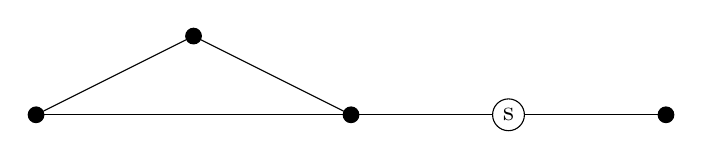
\begin{tikzpicture}
          % Draw the vertices
          \node[circle,draw,inner sep=2pt,fill] (v1) at (0,0) {};
          \node[circle,draw,inner sep=2pt,fill] (v2) at (2,1) {};
          \node[circle,draw,inner sep=2pt,fill] (v3) at (4,0) {};
          \node[circle,draw,inner sep=2pt] (s) at (6,0) {s};
          \node[circle,draw,inner sep=2pt,fill] (v4) at (8,0) {};

        
          % Draw the edges
          \draw (v1) -- (v2);
          \draw (v2) -- (v3);
          \draw (v3) -- (s);
          \draw (s) -- (v4);
          \draw (v1) -- (v3);
        
        \end{tikzpicture}
    \end{answer}

    \item Let $G = (V, E)$ be an undirected graph and let $s \in V$. Describe an efficient algorithm that checks if there is a cycle in G that contains s.
    \begin{answer}
    Perform DFS$(G, s)$ constructing DFS tree $T$ and marking tree edges
    Loop through non-tree edges and if there is an edge that has endpoint s (ie. back edge), then there is a cycle containing $s$
    Note: could also be accomplished with BFS.
    \end{answer}

    \item Makefiles specify the dependencies of programs during compilation. How can a Makefile be modeled as a graph? How can one compute an ordering of programs so that the programs are compiled under the dependency constraints.
    \begin{answer}
    A Makefile can be modeled as a directed graph. Nodes are programs. Edges encode dependencies, an edge from A to B, states that A is required to compile B. If a valid compilation graph, it should be a directed acyclic graph.
    
    We can run a topological sort to compile the dependencies first.
    \end{answer}

    \item  (CS374 SP23) Let G = (V, E) be a directed graph. Call a vertex of G good if it is in some cycle. Describe a linear-time algorithm to count the number of good vertices in G.
    \begin{answer}
    Compute the strong connected components (or the meta-graph) of G in linear time. A vertex is good iff it is in a strong connected component with at least two vertices. Thus, we add the sizes of all strong connected components that are of size at least two and output the sum. This second step is easy to compute in $O(|V|)$ time once we have the strong connected components as a list of lists. Thus the overall time is $O(|E| + |V|)$.

    \end{answer}

    \item Let G = (V, E) be a directed graph where the length of each edge is either 2 or 3. Describe a linear-time algorithm to find the shortest paths from a given node s.
    \begin{answer}
    We transform G into a graph G' = (V', E') with edge lengths 1 as follows. We replace each edge (u, v) of length 2 by a directed path with two edges connected u to v by introducing a new intermediate vertex. Similarly, we replace each edge of length 3 by a path with 3 edges between u and v by introducing 2 intermediate vertices. We then run BFS in G' from s to compute shortest path distances. Takes $O(|V|+|E|)$ time.
    \end{answer}
    
    
\end{enumerate}

\section{DP - Subsequences}
\begin{enumerate}
    \item Given arrays $A$ and $B$, find the subsequences $A'$ and $B'$ such that $A' \cdot B'$ is maximized.
    \begin{answer}
        Observe that we must have $|A'| = |B'|$. Let $MaxDot(i,j)$ be the maximum dot-product of subsequences from $A[i,\dots,|A|]$ and $B[j, \dots, |B|]$.
        \[
            MaxDot(i,j) = \begin{cases}
                0 & \text{$i > |A|$ or $j > |B|$} \\
                \max(A[i]\cdot B[j] + MaxDot(i+1,j+1), MaxDot(i+1,j), MaxDot(i,j+1)) & \text{o.w.}
            \end{cases}
        \]
        The recurrence can be memoized in a 2D array, with evaluation order decreasing in $i$ and $j$. This takes $O(|A||B|)$ time since each subproblem takes $O(1)$ time.
    \end{answer}
    \item Find the longest common palindromic subsequence of arrays $A$, $B$, and $C$.
    \begin{answer}
        See slides/recording please!
    %     Let $LCPS(i,j,k)$ denote the longest common palindromic subsequence generated from $A[i,\dots,|A|]$, $B[j, \dots, |B|]$, $C[k, \dots, |C|]$.
    %     \[
    %         \mkern-125mu LCPS(i,j,k) = \begin{cases}
    %             0 & \text{$i > |A|$ or $j > |B|$ or $k > |C|$} \\
    %             \max(LCPS(i+1, j+1, k+1) + 1, LCPS(i+1, j, k), LCPS(i,j+1,), LCPS(i,j,k+1)) & A[i] = B[j] = C[k] \\
    %             \max(LCPS(i+1, j, k), LCPS(i,j+1,), LCPS(i,j,k+1)) & \text{o.w.}
    %         \end{cases}
    %     \]
    %     The recurrence can be memoized in $O(|A||B||C|)$ time in decreasing $i,j,k$ order.
    \end{answer}
    \item The \textit{hamming distance} of two arrays $A_1$, $A_2$ of size $k$ is the number of bits that must be flipped to turn $A_1$ into $A_2$. Given array $A$ and array $B$, find the subsequence of $A$ with the smallest hamming distance to $B$.
    \begin{answer}
        Let $MinHam(i,j)$ denote the minimum hamming distance subsequence in $A[i,\dots,|A|]$ to $B[j,\dots,|B|]$.
        \[
            MinHam(i,j) = \begin{cases}
                \infty & i > n \wedge j \neq |B| + 1 \\
                0 & j = |B| + 1 \\
                \min((A[i] \oplus B[j]) + MinHam(i+1,j+1), MinHam(i+1,j)) & \text{o.w.}
            \end{cases}
        \]
        $MinHam$ can be memoized into a 2D array in $O(|A||B|)$ time in decreasing $j$, decreasing $i$ order.
    \end{answer}
    \item An element of array $A$ at index $i$ is \textit{proper} if $A[i] \geq \sum_{j=1}^{i-1} A[j]$. Find the longest sequence of proper elements.
    \begin{answer}
        Observe that it is never suboptimal to exclude a proper element from the answer subsequence, so we really just need to identify each element as proper or not. We could do this naively with a nested for loop, but a better solution is to use a single for loop to build array $A_s$ satisfying $A_s[i] = \sum_{j=1}^i A[j]$. Then, $A[i]$ is proper if $A[i] \geq A_s[i]$.  $A_s$ can be built in linear time with memoization, and it takes linear time to check all elements for properness, so the final runtime is $O(n)$.
    \end{answer}
    \item (Hard.) Find the subsequence of $A$ with the largest geometric mean (product of all the elements divided by count), and output the geometric mean of that sequence. 
    \begin{answer}
      We'll define $LGM(i)$ to be the largest geometric mean of $A[i, \dots, n]$, and the number of elements used to attain that value (i.e. its return value is a tuple). We have
        \[
            LGM(i) = \begin{cases}
                (1,0) & i = n + 1 \\
                \left(\frac{A[i] \cdot LGM(i+1)[0] \cdot LGM(i+1)[1]}{(LGM(i+1)[1] + 1)}, LGM(i+1)[1]\right) & \frac{A[i] \cdot LGM(i+1)[0] \cdot LGM(i+1)[1]}{(LGM(i+1)[1] + 1)} > LGM(i+1)[0] \\
                LGM(i+1) & \text{o.w.}
            \end{cases}
        \]
        This recurrence is a bit compilicated, but follows the same pattern as other recurrences: we decide, for each element, whether to include the element in the LGM or not. In this case, we just need more information to do that, hence returning a tuple.
        This can be memoized in $O(n)$ time, in decreasing $i$ order. There's an error in the recurrence though, can you spot it? We assumed all the elements of $A$ were positive. When wee see a negative element of $A$, we want to \textit{minimize} the arithmetic product of the remainder of the array, since a negative times a negative is positive. We actually need mutual recurrences, one for minimization and one for maximization:
        \[
            LGM(i) = \begin{cases}
                (1,0) & i = n + 1 \\
                \left(\frac{A[i] \cdot LGM(i+1)[0] \cdot LGM(i+1)[1]}{(LGM(i+1)[1] + 1)}, LGM(i+1)[1]+1\right) & \frac{A[i] \cdot LGM(i+1)[0] \cdot LGM(i+1)[1]}{(LGM(i+1)[1] + 1)} > LGM(i+1)[0] \wedge A[i] \geq 0 \\
                \left(\frac{A[i] \cdot SGM(i+1)[0] \cdot SGM(i+1)[1]}{(SGM(i+1)[1] + 1)}, SGM(i+1)[1]+1\right) & \frac{A[i] \cdot SGM(i+1)[0] \cdot SGM(i+1)[1]}{(SGM(i+1)[1] + 1)} > LGM(i+1)[0] \wedge A[i] < 0 \\
                LGM(i+1) & \text{o.w.}
            \end{cases}
        \]
        And then SGM is the mirror image:
        \[
            SGM(i) = \begin{cases}
                (1,0) & i = n + 1 \\
                \left(\frac{A[i] \cdot SGM(i+1)[0] \cdot SGM(i+1)[1]}{(SGM(i+1)[1] + 1)}, SGM(i+1)[1]+1\right) & \frac{A[i] \cdot SGM(i+1)[0] \cdot SGM(i+1)[1]}{(SGM(i+1)[1] + 1)} < SGM(i+1)[0] \wedge A[i] \geq 0 \\
                \left(\frac{A[i] \cdot LGM(i+1)[0] \cdot LGM(i+1)[1]}{(LGM(i+1)[1] + 1)}, LGM(i+1)[1]+1\right) & \frac{A[i] \cdot LGM(i+1)[0] \cdot LGM(i+1)[1]}{(LGM(i+1)[1] + 1)} < SGM(i+1)[0] \wedge A[i] < 0 \\
                SGM(i+1) & \text{o.w.}
            \end{cases}
        \]
    \end{answer}
\end{enumerate}

\section{DP - Subarrays}
\begin{enumerate}
    \item Compute the longest common subarray of $A$ and $B$.
    \begin{answer}
        Let $LCS(i,j)$ be the longest common subarray of $A[i,\dots,|A|]$ and $B[j,\dots,|B|]$. At each index, our recurrence has two options: start the common subarray here (if possible), or start somewhere later:
        \[
            LCS(i,j) = \begin{cases}
                0 & i > |A| \vee j > |B| \\
                \max(\max \{k : A[i,\dots,i+k] = B[j,\dots,j+k]\}, LCS(i+1,j), LCS(i,j+1)) & \text{o.w.}
            \end{cases}
        \]
        Let $\max$ of an empty set return $0$ so if there is no common subarray $LCS$ will return $0$. This can be memoized in a 2D array in decreasing $i$ and $j$ order in $O(n^3)$ time.
    \end{answer}
    \item Given an array $A$, partition $A$ into as few subarrays as possible such that the concatenation of digits in each subarray is prime. Assume you have access to an $O(1)$ black box for \texttt{IsPrime}.
    \begin{answer}
        Let $MinPrimes(i)$ be the minimum number of ways to partition $A[i,\dots,n]$ into subarrays of primes. The decision our recurrence needs to make is where to stop the current prime and start the next one:
        \[
            MinPrimes(i) = \begin{cases}
                0 & i = n + 1 \\
                \min_{i < m \leq n+1 : \texttt{IsPrime}(A[i,\dots,m-1])}\left(1 + MinPrimes(m)\right) & \text{o.w.}
            \end{cases}
        \]
        Let $\min_{\text{cond}}$ return $\infty$ if the condition cannot be satisfied, so that $MinPrimes$ will return $\infty$ if the array cannot be partitioned. $MinPrimes$ has $O(n)$ subproblems, each taking $O(n)$ time, so the final runtime is $O(n^2)$. Memoize in decreasing $i$ order.
    \end{answer}
\end{enumerate}

\section{DP - Optimization}
\begin{enumerate}
    \item At Willy Wonka's Chocolate Factory, Charlie|who is now remarkably jaded|wants to take as much chocolate as he can to resell. On his tour, Charlie will visit $n$ rooms, each with chocolate worth $C[i]> 0$. Rooms that are risky to steal from have $R[i] = 1$, else $R[i] = 0$. Given Charlie can only steal from $k$ risky rooms, what is the maximum amount of candy he can obtain?
    \begin{answer}
        At each room, Charline must make the decision to take candy or not, so our recurrence should take the maximum of each option. Let $MaxStolen(i,k)$ be the maximum amount of chocolate Charlie can steal from rooms $i,\dots,n$, given he can steal from $k$ more risky rooms. We can write this as
        \[
            MaxStolen(i,k) = \begin{cases}
                0 & i > n \\
                \max(C[i] + MaxStolen(i+1,k-1), MaxStolen(i+1,k)) & R[i] = 1 \wedge k > 0 \\
                MaxStolen(i+1,k) & R[i] = 1 \wedge k = 0 \\
                C[i] + MaxStolen(i+1,k) & o.w.
            \end{cases}
        \]
        The last case follows because we should always take chocolate if it's not risky. Yum! This can be memoized into an $O(nk)$ size array, each subproblem takes $O(1)$ time, so the final runtime is $O(nk)$. Evaluate in decreasing $i$ and increasing $k$ order. The final answer is $MaxStolen(1,k)$.
    \end{answer}
    \item (Hard.) Aaron wants to open $k$ gyms in Champaign, which can be represented as a 1D line of $n$ houses. Each gym will replace one house. Each house has a demand $D[i]$ for how much they want to use a gym. When a house has demand $D[i]$ and a gym is $m$ houses away, the house's demand for that gym is $D[i]/m$. Find the maximum demand Aaron can obtain.
    \begin{answer}
        Let $MaxDemand(i,k)$ be the maximum demand generated by $A[i,\dots,n]$ such that a gym replaces house $i$ and there are $k$ gyms remaining after this one.
        \[
            \mkern-100mu MaxDemand(i,k) = \begin{cases}
                \sum_{j=i+1}^{n}\frac{D[j]}{j-i} & k = 0 \\
                \max_{i + 1 \leq m \leq n} \left(\sum_{j=i+1}^{m-1} \frac{D[j]}{j-i}\left[\frac{D[j]}{j-i} < \frac{D[j]}{m-j}\right] + \sum_{j=i+1}^{m-1} \frac{D[j]}{m-j}\left[\frac{D[j]}{j-i} \geq \frac{D[j]}{m-j}\right] + MaxDemand(m,k-1)\right) & \text{o.w.}
            \end{cases}
        \]
        Here, $MaxDemand$ steps through all the gyms, deciding where to place each. We observe that if there are two gyms at $x_1$ and $x_2$, and $x_1 > x_2$, any gyms to the left of $x_1$ will never have more demand for $x_2$ than they will for $x_1$. Thus, when $MaxDemand$ decides where to place the next gym, it need only consider houses right of $i$ and left of $m$; for each of these houses, we compute their demand to each of the two gyms, and add the bigger one (a condition in brackets evaluates to $0$ when false and $1$ when true). The sums each take $O(n)$ time, and the outer max has $O(n)$ iterations, so each subproblem takes $O(n^2)$ time to solve. There are $O(nk)$ subproblems, so after memoization this takes $O(n^3 k)$ time to solve. The final answer can be returned by $MaxDemand(0,k)$ after adding a sentinel house at index $0$.
    \end{answer}
\end{enumerate}

\section{DP - Graphs}
\begin{enumerate}
    \item Sania is trying to infiltrate the Siebel Center for Computer Science to take all the free food she can. She starts off with a single key|Ryan's stolen iCard|which will get her inside the building. Once inside, the building is represented as a directed graph $G = (V, E)$. We can write $V = P \cup S$, where $P$ are publicly accessible rooms, and $S$ are staff accessible rooms. Some vertices may also contain a staff key left out that Sania can steal ($s(v) = 1$ if this is the case, else $s(v) = 0$) to gain access to staff accessible rooms. Each vertex offers $f(v)$ free food. What is the maximum amount of food Sania can steal?
    \begin{answer}
        When we see wanting to collect a lot of something, strongly connected components are a natural choice. We'll need to track the following information for each SCC: does it have a staff key, how much staff food is available, how much public food is available? This can all be computed for each SCC in $O(|V| + |E|)$ time with careful for loops, which we omit here. Once we have this, we can simply modify the standard longest path recurrence:
        \[
            \mkern-75mu MaxFood(s, k) = \begin{cases}
               s.staffFood + s.publicFood + \max_{v \in adj(s)}MaxFood(v, k = T \wedge s.staffKey) & k = T \wedge s.staffKey \\
               s.publicFood + \max_{v \in adj(s)}MaxFood(v, s.staffKey) & \text{o.w.}
            \end{cases}
        \]
        where $LP(s,k)$ is the longest path starting at $s$, where $k=T$ iff you have a staff key. For convenience, we let $\max$ over an empty set return $0$. This can be memoized just like standard longest path DP, and runtime stays $O(|V| + |E|)$.
    \end{answer}
    \item An NFA (with no $\epsilon$-transitions can be represented as a (not necessarily acylic) directed graph $G = (V, E)$, where edges are labeled with one or more symbols and represent transitions and vertices represent states. Let $\ell(e)$ denote the set of characters corresponding to the transition given by $e$. Given a start state $s$, string $w$, and array $A$ of accepting states, does the NFA accept $w$?
    \begin{answer}
        (Assume no $\epsilon$-transitions, otherwise the below does not work!)
        Let $Acc(t,i)$ be whether $M$ accepts $w[i,\dots,n]$ starting in state $t$. If $i = |w| + 1$, then we require $t$ to be an accept state, otherwise we require some transition to accept:
        \[
            Acc(t,i) = \begin{cases}
                t \in A & w = \epsilon \\
                \bigvee\limits_{u \in adj(t) : \texttt{label}(u) = w[i]} Acc(t, i+1) & \text{o.w.}
            \end{cases}
        \]
        We can precompute $t \in A$ for all $t$ in $O(|V|)$ time upfront, so the runtime is $O(|w|(|V| + |E|)$ following standard graph DP analysis. Observe that our recurrence only depends on bigger values of $i$, so we can evaluate in decreasing $i$ and any order for $v$.
    \end{answer}
\end{enumerate}

\section{Divide and Conquer}
\begin{enumerate}
    \item In a sorted array of distinct positive integers, is there an index $i$ such that $A[i] = i$?
    \begin{answer}
        Trick question! This can be solved in $O(1)$ time: if $A[1] = 1$, return true, else return false. Since the integers are distinct and positive, if $A[1] \neq 1$, then $A[1] > 1$, and $A[2] > 2$, and so on.
    \end{answer}
    \item Given array $A$, compute the 75th percentile value. Extend your algorithm to compute the $p$th percentile.
    \begin{answer}
        In $O(n)$ time we can compute the median (50th percentile), and build an array of all the values greater than the median. The median of this array is the 75th percentile value. This takes $O(n)$ time total. To compute the $p$th percentile, we can keep recursively computing medians of either the elements greater than or smaller than the previous median until we reach percentile $p$. Since $p$ is a constant between $0$ and $100$, this takes only $O(n)$ time.
    \end{answer}
    \item (Kinda hard.) Given an array $A$, two indices $i$ and $j$ are $k$-close if $|A[i] - A[j]| \leq k$. Report the number of $k$-close indicies.
    \begin{answer}
        Let's reformulate this problem as thinking of counting close points on the number line. With this idea in mind, we can develop a divide and conquer algorithm. Suppose we split the points by median. We know how many close points are in each half, so what additional information do we need to get the correct amount? We need to find out how many points are close to the median point (easy to do this|$O(n)$ scan), as well as how many points on the left are close to points on the right. This is harder, but can be accomplished with an $O(n\log n)$ time algorithm too: sort each side of points. Then, start at the rightmost point on the left, and find the rightmost point on the right that is still close; this is the $i$th point on the right, so there must be $i$ close pairs generated by this point on the left. Now move to the second-most-rightmost point on the left, and decrement $i$ to $i'$ until $i'$ is a right point close to the point on the left. Add $i'$ pairs generated by this point. Continue this process for all points on the left. This algorithm has a recurrence of $T(n) = 2T(n/2) + O(n\log n) = O(n\log^2 n)$. Can you spot how to do it in $O(n\log n)$? (Hint: we sort a lot...)
    \end{answer}
\end{enumerate}

\section{Graphs - Transformations and Shortest Paths}
\begin{enumerate}
    \item Given a directed graph $G = (V, E)$, a vertex is lighted if $\ell(v) = 1$. A path is safe if it has no more than three consecutive unlit vertices. Given a vertex $s$ and vertex $t$, what is the shortest lighted path from $s$ to $t$?
    \begin{answer}
        Build $G' = (V \times \{0,\dots,3\}, \{((u,i), (v,i+1) : i < 3 \wedge \ell(u) = 0\} \cup \{((u,i), (v,0)) : \ell(u) = 1\})$.
        The second part of each vertex tracks how many unlit vertices we've seen. By construction, all paths with more than $3$ consecutive unlit vertices lead to nowhere. Our final answer can be obtained by WFS from $s$, in $O(|V'| + |E'|) = O(|V| + |E|)$ time.
    \end{answer}
    \item Given a vertex $v$ is a graph with postive weights, what is the lightest cycle that includes $v$, if one exists?
    \begin{answer}
        Run Dijkstra from $v$, which gives $dist(v,t)$ for all $t$. If $dist(v,t) \neq \infty$ for at least one $t$ such that there is a $t \to v$ edge, return $\min_{t \to v}(dist(v,t) + w(t,v))$. This takes time dominated by Dijkstra's, which is $O(V\log V)$.
    \end{answer}
\end{enumerate}

\section{Reductions - Concepts}
For each statement below, select all claims that must be true if the statement is true regardless of the choice of the problem $X$.
\begin{enumerate}
    \item $X \leq_p \text{SAT}$: $X \in P$, $X \in NP$, $X$ is decidable, $X$ is undecidable
    \begin{answer}
        $X \in NP$ and $X$ is decidable must be true. Since $\text{SAT}$ is $NP$-complete, any problem
        in $NP$ can be reduced to it. Furthermore, since $NP$ is closed under reductions,
        we must have $X \in NP$. Since it is unknown if $P = NP$, we don't know if $X \in P$ or not.
        $X$ is decidable since it is in $NP$: recall that $X \in NP$ when there is a nondeterministic TM that
        solves (aka decides) it. Since $X$ is decidable, it cannot be undecidable.
    \end{answer}
    \item $\text{SAT} \leq_p X$: $X \in P$, $X \in NP$, $X$ is decidable, $X$ is undecidable
    \begin{answer}
        No claims must be true. It is possible to reduce $\text{SAT}$ to the following undecidable problem: $X = \{ \langle M \rangle : M~\text{accepts infinite strings}\}$ by building a nondeterministic turing machine $M$ which guesses a solution to a formula $\Phi$ and accepts only if that guess is correct. By definition, $M$ will only accept a string if there is a valid guess to solve $\Phi$, and we can construct an encoding for $M$ in polynomial time; thus $\langle M \rangle \in X \iff \Phi$ is satisfiable. Undecidable problems are not in $P$ or $NP$, so the first two statements need not be true, and clearly the third statement need not be true. But we also know that we can reduce $\text{SAT}$ to $\text{HP}$, which is decidable, so the fourth statement need not be true either.
    \end{answer}
    \item $X \leq_p \text{ShortestPath}$: $X \in P$, $X \in NP$, $X$ is decidable, $X$ is undecidable
    \begin{answer}
        $X \in P$ and $X$ is decidable must be true. Since $X$ is at most as hard as ShortestPath, a problem in $P$, we know that $X \in P$. This immediately implies $X$ is decidable, and therefore $X$ cannot be undecidable. Furthermore, since $X \in P$, then $X \in NP$.
    \end{answer}
    \item $X \implies HALT$: $X \in P$, $X \in NP$, $X$ is decidable, $X$ is undecidable
    \begin{answer}
        No claims must be true. Suppose $X$ is your favorite $NP$-hard problem, and build the following machine $M$:
        \begin{algorithmic}
            \Function{M}{$w$}
                \State Run algorithm for $X$ on $w$
                \State If the algorithm said yes, accept $w$
                \State Else, run forever
            \EndFunction
        \end{algorithmic}
        Now we've constructed $M$ so that $\langle M, w \rangle \in HALT$ only when $w \in X$. We can do this for any decidable problem $X$ (not just $NP$-hard), so we can't say for certain that $X \in P$ or $X \in NP$. We can also pick an undecidable $X$ though - recall all problems reduce to themselves, so we could pick $X = HALT$, and thus it need not be the case that $X$ is decidable or that $X$ is undecidable.
    \end{answer}
    \item $HALT \implies X$: $X \in P$, $X \in NP$, $X$ is decidable, $X$ is undecidable
    \begin{answer}
        $X$ must be undecidable. Since $HALT$ is undecidable, $X$ cannot be any easier.
    \end{answer}
\end{enumerate}

\noindent Determine whether each of the following claims are true or false.
\begin{enumerate}
    % \item If $X \in NP$, then $X$ is recursively enumerable
    \item If $X$ is regular, then $X \in NP$
    \begin{answer}
        True. Regular languages are in $P$, and $P \subseteq NP$.
    \end{answer}
    \item If $X$ is decidable, then $X \in NP$
    \begin{answer}
        False. $X$ may be decidable but require more time than $NP$ allows.
    \end{answer}
    \item If $X$ is undecidable, then $X \notin NP$
    \begin{answer}
        True. All problems in $NP$ are decidable.
    \end{answer}
    \item If $X$ is in $P$, then $X \leq_p Y$ for \textit{any} $Y \in P$
    \begin{answer}
        False. $Y$ may not be $P$-complete.
    \end{answer}
    \item If $X$ is $NP$-complete, then $Y \leq_p X$ for \textit{any} $Y \in NP$
    \begin{answer}
        True. $X$ is $NP$-complete.
    \end{answer}
\end{enumerate}

\noindent Briefly describe reductions to show each of the following statements.
\begin{enumerate}
    \item $3SAT \implies HALT$
    \begin{answer}
        Given $\Phi$, build TM $M$ which tries all possible variable assignments for $\Phi$, and loops forever if none of them work. Thus, $M$ halts only if $\Phi$ has a satisfying assignment, so we've reduced $3SAT$ to $HALT$.
    \end{answer}
    \item $SAT \leq_p CircuitSAT$
    \begin{answer}
        Convert the boolean expression into a circuit and pass it to $CircuitSAT$.
    \end{answer}
    \item $\{\langle G, s, t \rangle : \text{$G$ has a path from $s$ to $t$}\} \leq_p SAT$
    \begin{answer}
        Our reduction must run in polynomial time. We can reduce by computing whether $G$ has an $s \to t$ path in $O(|V| + |E|)$ time (which is polynomial). If some such path exists, we provide $x \vee \neg x$ to $SAT$, and if not, we provide $x \wedge \neg x$ to $SAT$. The reduction runs in polynomial time, and by construction, $SAT$ can only output yes when there is a $s \to t$ path in $G$.
    \end{answer}
\end{enumerate}

\noindent Select which of the following decision problems are $NP$-hard, and provide a short justification for your answer.
\begin{enumerate}
    \item Given a graph $G$, is there a simple (no repeated vertices) path of length $k$?
    \begin{answer}
        Setting $k=|V|-1$ makes this equivalent to the Hamiltonian Path problem, which we know is $NP$-hard, so this must also be $NP$-hard.
    \end{answer}
    \item Given a graph $G$, is there a path from $s$ to $t$?
    \begin{answer}
        This is not $NP$-hard. It can be solved in $O(|V| + |E|)$ time with BFS.
    \end{answer}
    \item Given an acyclic circuit $C$ and its inputs, what is the output?
    \begin{answer}
        This is not NP-hard. There are no cycles, so we can write a dynamic programmig algorithm to solve this problem in $O(|V| + |E|)$ time. 
    \end{answer}
    \item Given an acyclic circuit $C$, are there some inputs so that it will output $1$?
    \begin{answer}
        This is $NP$-hard. Construct a circuit for each clause of a 3CNF formula using or and not-gates, and join all the clause-circuits
        with and-gates. The resulting circuit has polynomial size and took polynomial time to build, and will output $1$ only when the input bits satisfy the 3CNF formula. This is a reduction from $3SAT$, which we know to be $NP$-hard.
    \end{answer}
    \item Given a graph with one node colored red, can the remainder of the graph be three-colored?
    \begin{answer}
        This is $NP$-hard. Given a graph $G$, just add a detached red vertex to it and run the above decision problem. The detached red vertex doesn't affect the colorability of the remainder of the graph, so if the remainder of our new graph is three-colorable, our original graph is three-colorable. This is a reduction from $3COLOR$ which is $NP$-hard.
    \end{answer}
\end{enumerate}

\noindent Select which of the following problems are decidable or undecidable, and provide a short justification for your answer.
\begin{enumerate}
    \item $\{\langle M \rangle : 0 \in L(M)\}$
    \begin{answer}
        Undecidable. We can reduce from $HALT$ by building $M'$ which accepts $0$ only if a simulation of $M$ on $w$ accepts. Alternatively, undecidability follows from Rice's theorem.
    \end{answer}
    \item $\{\langle M \rangle : M\text{ has at most 374 states}\}$
    \begin{answer}
        Decidable. We can simply read the encoding of $M$ and count the number of states it contains. This is no different than checking the length of an array.
    \end{answer}
    \item $\{\langle M \rangle : |L(M)| = 374\}$
    \begin{answer}
        Undecidable. We can reduce from $HALT$ by building $M'$ which accepts $373$ arbirarily chosen strings right away, and otherwise simulates $M$ on $w$ and accepts a $374$th string only if the simulation accepted. Alternatively, undecidability follows from Rice's theorem.
    \end{answer}
    \item $\{\langle M \rangle : M\text{ halts on all inputs}\}$
    \begin{answer}
        Undecidable. This should be clear since this is a stronger statement than the undecidable halting problem. We can reduce from $HALT$ by building $M'$ which runs $M$ on $w$, and if $M$ halted on $w$, $M'$ halts (it can either accept or reject at this point, we'll choose to always accept).
    \end{answer}
    \item $\{\langle M, w, t \rangle : M\text{ halts on $w$ in at most $t$ steps}\}$
    \begin{answer}
        Decidable. Simulate $M$ and stop after $t$ steps. Since $t$ is always a finite number,
        this always terminates and it is easy to check what state $M$ is in after each step
        and accept/reject appropriately.
    \end{answer}
\end{enumerate}

\noindent Did you notice any pattern about the undecidability questions above?
\begin{answer}
    Asking things about the language of a machine, or its behavior on certain inputs, is usually undecidable (unless we can bound running time to avoid the halting problem), whereas asking things about the structure of the machine (i.e. its states) is decidable.
\end{answer}
% 10 questions (mostly conceptual)

\section{Undecidability Reductions}
Provide a proof that each of the following languages is undecidable (assume $M$ is always a TM). Do not use Rice's theorem.
\begin{enumerate}
    \item $L = \{\langle M \rangle : M~\text{accepts all even-length strings}\}$
    \begin{answer}
        We'll show $HALT \implies L$. That is, we want to find some function $f$ so that
        $\langle M, w \rangle \in L \iff f(\langle M, w\rangle) \in L$. This means $f$ should build
        a machine $M' = f(\langle M, w \rangle)$ so that $M'$ only accepts all even-length strings
        when $M$ halts on $w$. One way we can do this is by only accepting \textit{any} strings if $M$ halts on $w$, and accepting all strings after $M$ halts on $w$. That looks like the following machine:
        \begin{algorithmic}
            \Function{M'}{$x$}
                \State Run $M$ on $w$
                \State Accept $x$
            \EndFunction
        \end{algorithmic}
        Now we argue $\langle M, w \rangle \in L \iff f(\langle M, w\rangle) \in L$:
        \begin{itemize}
            \item $(\implies)$: Suppose $M$ halts on $w$. Then $M'$ reaches the second line, and so it accepts all strings, which include all even-length strings.
            \item $(\impliedby)$: By contrapositive, it is equivalent to prove that if $M$ does not halt on $w$, then $M'$ does not accept all even length strings. If $M$ does not halt on $w$, then $M'$ never reaches the second line, and so it accepts no strings, and thus does not accept all even-length strings.
        \end{itemize}
        Since $f$ is computable, we've shown $HALT \implies L$, which means $L$ is undecidable.
    \end{answer}
    \item $L = \{\langle M \rangle : |L(M)| \geq 1 \}$
    \begin{answer}
        We'll show $HALT \implies L$. We want to find $f$ so that 
        $\langle M, w \rangle \in L \iff f(\langle M, w \rangle) \in L$. This means $f$ should build machine $M'$ so that $M'$ accepts at least one string only if $M$ halts on $w$. We can do this by following the standard procedure of building $M'$ which runs $M$ on $w$ and uses $M$'s action as a gate to control whether $M'$ it belongs to $L$:
        \begin{algorithmic}
            \Function{M'}{$x$}
                \State Run $M$ on $w$
                \State Accept $x$
            \EndFunction
        \end{algorithmic}
        Now we argue $\langle M, w \rangle \in L \iff f(\langle M, w\rangle) \in L$:
        \begin{itemize}
            \item $(\implies)$: Suppose $M$ halts on $w$. Then $M'$ reaches the second line, and so it accepts all strings, which means $|L(M')| \geq 1$.
            \item $(\impliedby)$: By contrapositive, it is equivalent to prove that if $M$ does not halt on $w$, then $L(M') < 1$ (i.e. $L(M') = 0$). If $M$ does not halt on $w$, $M'$ never reaches the second line, and so does not accept any strings, so the claim is true.
        \end{itemize}
        Since $f$ is computable, we've shown $HALT \implies L$, which means $L$ is undecidable.
    \end{answer}
    \item $L = \{\langle M, w \rangle : M~\text{accepts $w$}\}$
    \begin{answer}
        First, note that the $w$ here doesn't have to be the same $w$ is in $HALT$, which is what we'll reduce from to show $HALT \implies L$. We'll choose $w=1$, and use $f$ to build a machine $M'$ which accepts $1$ only when $M$ halts on $w$:
        \begin{algorithmic}
            \Function{M'}{$x$}
                \State Run $M$ on $w$
                \State Accept $x$
            \EndFunction
        \end{algorithmic}
        Now we argue $\langle M, w \rangle \in L \iff f(\langle M, w\rangle) \in L$:
        \begin{itemize}
            \item $(\implies)$: When $M$ halts on $w$, then $M'$ reaches the second line and accepts all strings, including $1$.
            \item $(\impliedby)$: By contrapositive. When $M$ does not halt on $w$, $M'$ never reaches the second line, and never accepts any strings, and so does not accept $1$.
        \end{itemize}
        Since $f$ is computable, we've shown $HALT \implies L$, which means $L$ is undecidable.
    \end{answer}
    \item $L = \{\langle M, w, x \rangle : M~\text{accepts one of $w$ or $x$, but not both}\}$
    \begin{answer}
        Recall that if $\overline{L}$ is undecidable, then $L$ must be too. We'll use this fact and show that $HALT \implies \overline{L}$. We need to find $f$ and two strings $w,x$ so that $\langle M, w \rangle \in HALT \iff f(\langle M, w \rangle) \in \overline{L}$. $f$ will set $w=w$ and $x=1$, and needs to build some machine $M'$ so that $M'$ only accepts both $w$ and $x$ if $M$ halts on $w$. We can use the gating idea from before, and \textit{always} accept $x$, and then only accept $w$ when $M$ halts on it:
        \begin{algorithmic}
            \Function{M'}{$z$}
                \If{$z = x$}
                    \State Accept $z$
                \EndIf
                \State Run $M$ on $w$
                \State Accept $z$
            \EndFunction
        \end{algorithmic}
        Now we argue $\langle M, w \rangle \in HALT \iff f(\langle M, w \rangle) \in \overline{L}$:
        \begin{itemize}
            \item $(\implies)$: Suppose $M$ halts on $w$. Then $M'$ reaches the last line and accepts all strings, so $M'$ accepts both $w$ and $x$.
            \item $(\impliedby)$: By contrapositive. Suppose $M$ does not halt on $w$. Then $M'$ only accepts $x$ because it never reaches the last line, so $M'$ accepts $x$ but not $w$.
        \end{itemize}
        Since $f$ is computable, we've shown $HALT \implies L$, which means $L$ is undecidable.
    \end{answer}
    \item $L = \{\langle M \rangle : M~\text{runs for more than $n$ steps on some input of size $n$}\}$
    \begin{answer}
        The ``gating'' we've been doing before needs a little bit of modification here before we can use it. Consider the following machine $M'$ created reducing $HALT$ to $L$:
        \begin{algorithmic}
            \Function{M'}{$x$}
                \State Run $M$ on $w$
                \State Accept $x$
            \EndFunction
        \end{algorithmic}
        If $M$ does not halt on $x$, then $M'$ runs forever on all inputs, so $M' \in L$, which isn't what we want. We can fix this by tracking how many steps we've run $M$ for, and accepting $x$ when $|x|$ is equal to the number of steps we've taken so far:
        \begin{algorithmic}
            \Function{M'}{$x$}
                \State Run $M$ on $w$. At each step, if $|X| = \text{\# steps taken so far}$, accept $x$
                \State Accept $x$
            \EndFunction
        \end{algorithmic}
        Now if $M$ does not halt on $x$, it accepts all strings of length $n$ in exactly $n$ steps, so $\langle M' \rangle \notin L$. But if $M$ does halt on $x$ in $k$ steps, $M'$ accepts all strings of length $n \leq k$ in $n$ steps, and all strings of length $n' > k$ in $k$ steps, so $\langle M' \rangle \notin L$. We can observe that running forever fixes this, so our final reduction $f$ from $HALT$ to $L$ will be to construct the following machine $M'$:
        \begin{algorithmic}
            \Function{M'}{$x$}
                \State Run $M$ on $w$. At each step, if $|X| = \text{\# steps taken so far}$, accept $x$
                \State Loop forever
            \EndFunction
        \end{algorithmic}
        Now we argue $\langle M, w \rangle \in HALT \iff f(\langle M, w \rangle) \in L$:
        \begin{itemize}
            \item $(\implies)$: Suppose $M$ halts on $w$. It halts in some finite number of steps, call it $k$. Then $M'$ reaches the second line and runs forever, so there is some $x$ s.t. $|x| > k$ and $M'$ will run forever on it, so $\langle M' \rangle \in L$.
            \item $(\impliedby)$: By contrapositive. Suppose $M$ does not halt on $w$. Then $M'$ stays on the first line and accepts all strings of length $n$ in exactly $n$ steps, so $\langle M' \rangle \notin L$.
        \end{itemize}
        Since $f$ is computable, we've shown $HALT \implies L$, which means $L$ is undecidable.
    \end{answer}
    \item $L = \{\langle M \rangle : L(M) \text{ is regular}\}$
    \begin{answer}
        Once again, we'll show $HALT \implies L$ with a reduction $f$. The simpliest reduction we could make is for $f$ to build the following machine $M'$:
        \begin{algorithmic}
            \Function{M'}{$x$}
                \State Run $M$ on $w$
                \State Accept $x$
            \EndFunction
        \end{algorithmic}
        Unfortunately, if $M$ does not halt on $w$, $L(M') = \emptyset$ which is regular. We need to add something before we run $M$ on $w$ so that $L(M')$ only becomes regular if $M$ halts on $w$. We can do this using our favorite irregular language $I = \{0^n 1^n : n \geq 1 \}$:
        \begin{algorithmic}
            \Function{M'}{$x$}
                \State If $x = 0^n1^n$ for some $n$, accept
                \State Run $M$ on $w$
                \State Accept $x$
            \EndFunction
        \end{algorithmic}
        Now we argue $\langle M, w \rangle \in HALT \iff f(\langle M, w \rangle) \in L$:
        \begin{itemize}
            \item $(\implies)$: Suppose $M$ halts on $w$. Then $M'$ reaches the third line and accepts all strings, so $L(M') = \Sigma^*$ which is regular, so $\langle M' \rangle = f(\langle M, w \rangle) \in L$.
            \item $(\impliedby)$: Suppose $M$ runs forever on $w$. Then $M'$ never reaches the third line, and only accepts strings of the form $0^n 1^n$, so $L(M') = I$, which is irregular. Thus $\langle M' \rangle = f(\langle M, w \rangle) \notin L$.
        \end{itemize}
        Since $f$ is computable, we've shown $HALT \implies L$, which means $L$ is undecidable.
    \end{answer}
    \item $L = \{\langle M \rangle : L(M) \text{ is  not regular}\}$
    \begin{answer}
        Note that $\overline{L} = \{\langle M \rangle : L(M) \text{ is regular}\}$, which we showed was not decidable. Therefore $L$ cannot be decidable.
    \end{answer}
    
    % \item $L = \{\langle M \rangle : \}$
\end{enumerate}

\noindent We've seen that questions about the languages of Turing machines are typically undecidable. This is not the case for NFAs and DFAs: most questions are decidable. Provide an algorithm to decide each of the following languages (assume $M$ is always a DFA and $N$ an NFA).
\begin{enumerate}
    \item $L = \{\langle M, n \rangle : \text{$M$ accepts all binary strings of length $n$}\}$
    \begin{answer}
        There are $2^n$ binary strings of length $n$. Run $M$ on all of them, and if every one is accepted, accept $M$. This takes finite time, and so decides $L$.
    \end{answer}
    \item $L = \{\langle M, w \rangle : \text{$M$ accepts $w$}\}$
    \begin{answer}
        Just as above, run $M$ on $w$, and accept if $M$ accepted $w$. This procedure takes finite time (all DFAs/NFAs halt!), so it decides $L$.
    \end{answer}
    \item $L = \{\langle M, w \rangle : \text{$M$ accepts some string ending in $012$}\}$
    \begin{answer}
        Consider $M$ to be a graph $G$ where states are vertices, and transitions are labeled edges. In the reverse of $G$, check if there is a path starting from any accept state to a start state, where the first three edges in the path are labeled $2$, $1$, and $0$|if so, this path corresponds to some string that is accepted by $M$ ending in $012$. There are finitely many possible paths, so this algorithm runs in finite time and decides $L$.
    \end{answer}
    \item $L = \{\langle N \rangle : \text{All strings accepted by $N$ begin with a $1$}\}$
    \begin{answer}
        First convert $N$ to a DFA. From the single start state of this DFA, check that there are no paths to an accept state that begin with a character that is not $1$|if there are, reject. There are finitely many possible paths to consider, so this algorithm decides $L$.
    \end{answer}
    \item $L = \{\langle N, w \rangle : \text{All computations by $N$ on $w$ lead to acceptance}\}$
    \begin{answer}
        Simulate all possible computations, rejecting if any of them lead to a reject state; otherwise, accept at the end. There are finitely many possible computations, so this terminates and decides $L$.
    \end{answer}
\end{enumerate}
% 10 questions

\section{NP-Hardness Reductions}
Prove that each problem is NP-Hard. Problems denoted (*) are more challenging than average.
%3SAT 
\begin{enumerate}
    \item A SAT formula is \textit{mostly-satisfiable} if there is exactly one variable which, after being removed, results in the formula becoming satisfiable. Determine if a formula $\Phi$ is mostly-satisfiable.
    \begin{answer}
        The obvious reduction here is from SAT.
        Our goal is to add an additional variable $x$ to $\Phi$ so that $x$ must be removed to make $\Phi$ satisfiable. This way, when $x$ is removed from our new expression (call it $\Phi'$), the satisfiability is only dependent on the satisfiability of $\Phi$. Let $\Phi' = (\Phi) \wedge (x \wedge \neg x)$. This can clearly be constructed in polynomial time. Now we argue $\Phi'$ is mostly-satisfiable iff $\Phi$ is satisfiable:
        \begin{itemize}
            \item $(\implies)$: Suppose $\Phi$ is satisfiable. After removing $x$ from $\Phi'$, $\Phi' = \Phi$, so $\Phi'$ is satsifiable.
            \item $(\impliedby)$: Suppose $\Phi'$ is mostly-satisfiable. By construction of $\Phi'$, $\Phi'$ is not satisfiable because the clause $(x \wedge \neg x)$ cannot be satisfied regardless of choice of $x$. Thus, $x$ must be removed for $\Phi'$ to be satisfiable. After removing $x$, $\Phi'$ becomes satisfiable, and after removing $x$, $\Phi' = \Phi$, so we conclude $\Phi$ is satisfiable.
        \end{itemize}
        Since this reduction runs in polynomial time, we conclude $SAT \leq_p MostlySatisfiable$, so $MostlySatisfiable$ is $NP$-hard. $NP$-completeness follows similarly from the proof of $SAT$'s $NP$ membership.
    \end{answer}
    \item (*) Xavier thinks microwaves are too complicated, so he's set out to design his own. He doesn't want to worry about starting a timer on the microwave, so he's devised the following strategy: each food's box will specify any number of variables $v_1, \dots, v_n$, as well as any number of linear constraints (i.e. $v_1 + v_2 \le 2$ or $v_1 \geq v_n$) on a QR code the microwave will scan. Xavier's microwave will try to assign each $v_i$ to either $0$ or $1$ while satisfying the provided constraints and maximizing $\sum v_i$, the cooking time (since it's better to overcook than undercook!). If the microwave can't figure out how to cook the food, it will just turn off.
    \begin{answer}
        We want to take a 3SAT formula $\Phi$ and encode it as a set of constraints. The first constraint we'll encode is that every variable in $\Phi$ must be either true or false. For a variable $x_i$ in $\Phi$, create two variables for the microwave (called $x_i$ and $\neg x_i$), and add the constraints $x_i + \neg x_i \leq 1$ and $x_i + \neg x_i \geq 1$. Now we want to encode each clause of $\Phi$ as a constraint: for a clause $(q_i \wedge q_j \wedge q_k)$ add the constraint $q_1 + q_2 + q_3 \geq 1$ where $q_i$ corresponds to either $x_i$ or $\neg x_i$ depending on the clause, and similar for $q_j$ and $q_k$. There are only polynomially many constraints to construct, so this reduction takes polynomial time. Now we argue that $\Phi$ is satisfiable iff the microwave will turn on.
        \begin{itemize}
            \item $(\implies)$. Consider an arbitrary satisfying assignment to $\Phi$. Every variable is set to either true or false in the assignment, so for all $i$, the constraints $x_i + \neg x_i \leq 1$ and $x_i + \neg x_i \geq 1$ are satisfied. Additionally, every clause is satisfied, so some term in each clause is true, so all of the $q_1 + q_2 + q_3 \geq 1$ constraints are satisfied. Thus, the satisfying assignment corresponds to a choice of variables satisfying the constraints given to the microwave, so it will turn on.
            \item $(\impliedby)$. Suppose the microwave turns on. For each variable pair $(x_i, \neg x_i)$, this means the constraints $x_i + \neg x_i \leq 1$ and $x_i + \neg x_i \geq 1$ are satisfied. This implies exactly one of $x_i$ or $\neg x_i$ must be set to $1$ (i.e. $x_i$ must either be true or false). We also know that each clause-constraint $q_i + q_j + q_k \geq 1$ is satisfied, and by construction, since each $q_i, q_j, q_k$ map back to a variable in the original clause, the satisfaction of a clause-constraint means the clause will be satisfied. Since all clauses are satisfied, $\Phi$ is satisfiable.
        \end{itemize}
        Since this reduction runs in polynomial time, we conclude $3SAT \leq_p Microwave$, so $Microwave$ is $NP$-hard. We can show $NP$-completeness by writing a polynomial-time algorithm to check that a set of variable assignments satisfies the microwave constraints. Maybe microwaves are hard after all!
    \end{answer}
% \end{enumerate}
% CircuitSAT
% \begin{enumerate}
    \item A boolean circuit $C$ is \textit{kinda-ok} if, after switching exactly one or-gate to an and-gate (or vice versa), the circuit is satisfiable. Given a circuit $C$, is it kinda-ok?
    \begin{answer}
        We can apply a similar idea as problem (1), where we control which gate must be switched. Given a circuit $C$, we'll build circuit $C'$ as follows: add an and-gate with inputs $x$ and $\neg x$ for a new variable $x$. Set the output gate to be another new and-gate, with inputs of the output gate of $C$, and the output of the and-gate we just built for $x$ and $\neg x$. What we built looks like this:
        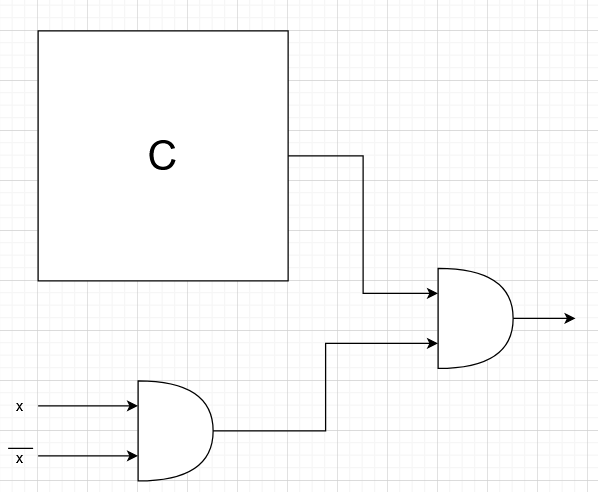
\includegraphics[width=3in]{figures/circuit.png}\\
        Now we argue that $C$ has a satisfying assignment iff $C'$ is kinda-ok.
        \begin{itemize}
            \item $(\implies)$: Suppose $C$ has a satisfying assignment. Then the output of gate of circuit $C$ can be set to $1$. The and gate for $x$ and $\neg x$ will have an output of $0$, so by switching the output gate of $C'$ to an or-gate, $C'$ will output $1$.
            \item $(\impliedby)$: Suppose $C'$ is kinda-ok. Since $x$ and $\neg x$ cannot both be $1$ at the same time, the output and-gate will output $0$. Flipping any gate in $C$ will not change this, so the gate flipped for $C'$ to be kinda-ok must be either of the and-gates we added. In either case, the result is that $C'$'s output gate will output the same thing as $C$'s output gate. Since $C'$ is kinda-ok, this means after the flip $C'$ outputs $1$, and so $C$ must output $1$. Thus $C$ is satisfiable.
        \end{itemize}
        This reduction can be performed in polynomial time since we're adding a constant amount of information to the circuit. Thus $CircuitSAT \leq_p KindaOk$ so $KindaOK$ is $NP$-hard. $NP$-completeness follows similarly to the proof of $CircuitSAT$'s $NP$-completeness.
    \end{answer}
    % \item Xavier is continuing his microwave adventure. He wants to simplify the circuitry of his microwave as much as possible, and so given two circuits $C$ and $C'$ he wants to determine if they're equivalent.
% \end{enumerate}
% Independent set
% \begin{enumerate}
    \item The University of Illinois has decided to open its own zoo! The can choose from a list of $n$ animals, and have access to a list of tuples $(i,j)$, which mean animal $i$ would eat animal $j$ if given the opportunity. Unfortunately, the only animals available to them have a tendency to escape, so they want to find the largest subset of animals that will not eat one another if they escape (called a \textit{safe} subset).
    \begin{answer}
        When we see a problem about finding a maximum sized set with some separation, independent set is a good choice. In independent set, we want to pick the largest subset of non-adjacent vertices, so we want to map adjacent to animals that eat each other so that the set of animals returned by $Zoo$ will be a set of nonadjacent vertices. In particular, our reduction is as follows: given a graph $G$, for each vertex $v_i$, create an animal $i$; for each edge $(v_i, v_j)$ tell the university that $i$ would eat $j$ if given the chance. Denote $M$ to be the size of the maximum independent set in $G$, and $S$ to be the size of the maximum safe set in the zoo input we constructed. We'll show that $M = S$ by showing $M \leq S$ and $M \geq S$:
        \begin{itemize}
            \item $M \leq S$: Let $\mathcal{M}$ be the maximum independent set in $G$. No two vertices in this set are adjacent, and by construction, this means that for any $v_i, v_j \in \mathcal{M}$, $i$ will not eat $j$ so $i$ and $j$ can both be added to a safe set. Since this holds for all $v_i, v_j \in \mathcal{M}$, we can construct a safe set of size $M$. This will be no better than the size of the largest safe set, so $M \leq S$.
            \item $M \geq S$: Let $\mathcal{S}$ be the maximum size safe set in $G$. No two animals in this set will eat each other, so the vertices corresponding to these animals are all non-adjacent, so we can construct an independent set in $G$ using the vertices corresponding to the animals in the safe set. This set has size $S$, which cannot be any better than the maximum size independent set, so $S \leq M$.
        \end{itemize}
        This reduction takes polynomial time, so $IndependentSet \leq_p Zoo$ and $Zoo$ is $NP$-hard.
    \end{answer}
    \item A set of vertices is \textit{mostly independent} if each vertex in the set is adjacent to at most one other vertex in the set. Compute the size of the largest mostly independent set of vertices.
    \begin{answer}
        Our goal here is to control the adjacent vertices so that we can reduce from $MaxIndependentSet$. We'll perform the following reduction: for each vertex in $G$, add a new vertex and connect it to the original vertex. That is, $V' = V \cup \{1, \dots, |V|\}$ and $E' = E \cup \{v_i i : i \in \{1,\dots, |V|\}\}$. For convenience, let $A = \{1, \dots, |V|\}$. Now we'll argue that there is a maximal mostly independent set in $G'$ which contains every vertex in $A$. Consider an arbitrary maximum mostly independent set $\mathcal{M}$, and $v_i \in \mathcal{M} \setminus A$. If any neighbor $v_j$ of $v_i$ is also in $\mathcal{M}$, we know that $i \notin \mathcal{M}$, so we can set $\mathcal{M}' = \mathcal{M} - v_j + i$, which has the same size. If no neighbor $v_j$ of $v_i$ is in $\mathcal{M}$, then $i \in \mathcal{M}$, otherwise $\mathcal{M}$ would not be maximal. We can repeatedly do the $\mathcal{M'}$ finding procedure above to find a maximal mostly independent set that contains all vertices in $A$. Let $k$ be the size of the maximum independent set in $G$, now we argue that $G$ has an independent set of size $K$ iff $G'$ has a mostly independent set of size $k + |V|$.
        \begin{itemize}
            \item $(\implies)$. For an independent set $I$, let $\mathcal{M} = I \cup A$. This is mostly-independent because no vertices in $I$ are adjacent to one another, and all vertices in $A$ are adjacent to exactly one vertex in $G$. $\mathcal{M}$ has size $|I| + |A| = k + |V|$.
            \item $(\impliedby)$. Consider a mostly independent set $\mathcal{M}$. By the above, we can assume it contains all vertices in $A$. As a result, any vertex $v \in M$, where $v \in G$ will not be adjacent to any other vertices in $G$: it is already adjacent to some vertex in $A$. After removing $A$ from $\mathcal{M}$, we get a set of vertices in $G$ which must be independent, and has size $k + |V| - |A| = k$.
        \end{itemize}
        Since this reduction runs in polynomial time, we conclude that $MaxIndependentSet \leq_p MostlyIndependent$, so $MostlyIndependent$ is $NP$-hard.
    \end{answer}
% \end{enumerate}
% Clique
% \begin{enumerate}
    \item A clique is \textit{light} if it contains at most $n/2$ vertices. Find the size of the largest light clique in $G$.
    \begin{answer}
        The natural problem to reduce from here is $k$-clique. Given a graph $G$, we want to find a graph $G'$ such that $G'$ has a $k$-clique iff $G$ has a $k$-clique, but subject to the additional constraint that $k < |V(G')|/2$. We can do this by letting $G'$ consist of two copies of $G$, neither connected to the other. A clique cannot have vertices in both copies, so any clique in $G'$ has size at most $|V(G')|/2$. Now it only remains to show that $G$ has a $k$-clique iff $G'$ has a $k$-clique:
        \begin{itemize}
            \item $(\implies)$. Suppose $G$ has a $k$-clique. Since $G'$ contains two copies of $G$, this $k$-clique is also a clique in one of these copies, and is thus a $k$-clique in $G'$.
            \item $(\impliedby)$. Suppose $G'$ has a $k$-clique. Since $G'$ contains two disjoint copies of $G$, the clique must lie entirely in one copy of $G$, so it's necessarily a $k$-clique in $G$.
        \end{itemize}
        From the above, we can conclude that the size of the largest light clique in $G'$ is the same as the size of the largest clique in $G$. Since it takes polynomial time to build $G'$, we've shown $Clique \leq_p LightClique$, so $LightClique$ is $NP$-hard.
    \end{answer}
% \end{enumerate}
% Vertex cover
% \begin{enumerate}
    \item Hans is planning his wedding and wants to seat guests with similar interests at the same table. His guests are eccentric, and each have exactly two interests. Compute the minimum number of tables Hans must rent, assuming each guest must sit down.
    \begin{answer}
        Since each guest must sit down, and we want the minimum number of tables so that each guest can sit down, it seems like guests might be similar to edges in the $VertexCover$ problem, so we'll reduce from $VertexCover$.
        Given a graph $G$, build a guest list as follows: each edge $uv \in E$ is a guest, with interests $u$ and $v$. We argue that $G$ has a vertex cover of size $k$ iff $k$ tables can be used for the wedding.
        \begin{itemize}
            \item $(\implies)$. Suppose $G$ has a vertex cover $C$ of size $k$. For each vertex in $C$, create a table. Since $C$ is a vertex cover, for every edge (guest), there must be some vertex (table) that covers it, so assign all guests to the table corresponding to their covered endpoint (if both endpoints are covered, pick arbitrarily). Since $C$ is a cover, all guests will be seated using $k$ tables.
            \item $(\impliedby)$. Suppose hans can seat the guests with $k$ tables. At each table, guests all must share some common interest corresponding to one of their endpoints. For each table, add the vertex corresponding to the common interest (if multiple, pick arbitrarily) to a cover $C$; since all guests at this table share this interest, their corresponding edges will be covered by $C$. Because we do this procedure for all tables, $C$ is a vertex cover of size $k$.
        \end{itemize}
        Since our reduction runs in polynomial time, we conclude that $VertexCover \leq_p WeddingPlanning$ and $WeddingPlanning$ is $NP$-hard. Unfortunate!
    \end{answer}
    \item (*) A vertex cover $C$ of size $k$ is \textit{balanced} if it can be partitioned into sets $C_1$ and $C_2$ so that $C_1 \cup C_2 = C$, $C_1 \cap C_2 = \emptyset$, $|C_1| = |C_2|$ and there are no edges between vertices in $C_1$ and $C_2$. Compute the size of the smallest balanced vertex cover.
    \begin{answer}
        The disjointness and equal size constraints sound similar to question (7), so let's try the same reduction, but this time from $VertexCover$. Given a graph $G$, let $G'$ contain two copies of $G$, not connected to each other. We now argue that $G$ has a vertex cover of size $k$ iff $G'$ has a balanced vertex cover of size $2k$.
        \begin{itemize}
            \item $(\implies)$. Suppose $G$ has a smallest vertex cover of size $k$. A vertex cover of $G$ must cover both copies of $G$, and since using $k$ covers one copy most efficiently, we can use use $2k$ vertices to cover both copies most efficiently|$k$ for each copy. Thus $G'$ has a minimum balanced vertex cover of size $2k$.
            \item $(\impliedby)$. Suppose $G'$ has a minimal balanced vertex cover of size $2k$. By definition, we can partition this into sets $C_1, C_2$ each of size $k$. We argue that we can partition so that $C_1$ only contains vertices from the first copy of $G$, and $C_2$ from the second: suppose otherwise. Then, without loss of generality $C_1$ covers all of $G$ using $k' < k$ vertices. This contradicts that the balanced vertex cover is minimal, since we could use $k'$ vertices in place of $C_2$ so that there is a balanced vertex cover of size $2k' < 2k$. Since this is a contradiction, we can partition $C$ so that $C_1$ only contains vertices in the first copy of $G$ and $C_2$ from the second. Since $C$ is a vertex cover, then $C_1$ must cover the first copy of $G$, so $C_1$ is a vertex cover of size $k$ for $G$. It must be minimal: if not, we could've found a smaller balanced vertex cover using the reasoning above.
        \end{itemize}
        Since this reduction runs in polynomial time, we conclude $VertexCover \leq_p BalancedVertexCover$ and thus $BalancedVertexCover$ is $NP$-hard.
    \end{answer}
% \end{enumerate}
% Ham-cycle/ham-path
% \begin{enumerate}
    \item Given a graph $G$ with red and white edges, \textit{candy cane path} alternates between red and white edges. Compute the length of the longest candy cane path.
    \begin{answer}
        This sounds a lot like Hamiltonian Path / Longest Path, so let's reduce from that. Given a graph $G$, we'll construct $G'$ by expanding each vertex into two as below: \\
        \includegraphics[width=6in]{figures/Screenshot 2023-11-22 at 14-21-59 Excalidraw — Collaborative whiteboarding made easy.png} \\
        where the inner edge is colored red, and all other edges are colored white.
        Now we argue that $G$ has a path of length $k$ iff $G'$ has a candy-cane path of length $2k$.
        \begin{itemize}
            \item $(\implies)$. Suppose $G$ has a path $P = v_1\cdots v_k$ of length $k$. Each vertex $v_i$ in this path corresponds to two vertices $v_i^{(\text{left})}$ and $v_i^{(\text{right})}$ in $G'$ with a red edge between them. Let $P' = v_1^{(\text{left})}v_1^{(\text{right})}\cdots v_1^{(\text{left})}v_1^{(\text{right})}$. $P'$ is a candy-cane path: every $v_i^{(\text{left})} \to v_i^{(\text{right})}$ edge is red, and every $v_i^{(\text{right})} \to v_i^{(\text{left})}$ edge is white.
            \item $(\impliedby)$. Suppose $G'$ has a candy-cane path $P = w_1 \dots w_{2k}$ of length $2k$. By construction, if the $w_{i} \to w_{i+1}$ edge is red, then $w_i = v^{(\text{left})}$ and $w_{i+1} = v^{(\text{right})}$ for some $v \in V(G)$. Thus we can compress all these adjacent pairs, halving the length of $P$ and obtaining a path of length $k$ in $G$.
        \end{itemize}
        From the above, we conclude that $G$ has a Hamiltonian path iff $G'$ has a candy-cane path of length $2(|V| - 1)$. Since the reduction runs in polynomial time, $HamPath \leq_p CandyCanePath$ and we conclude $CandyCanePath$ is $NP$-hard.
    \end{answer}
    \item A \textit{half-assed Hamiltonian cycle} visits at least $(1/100)$th of the vertices of a graph $G$. Compute the length of the longest half-assed Hamiltonian cycle. (Hint: start with $1/2$).
    \begin{answer}
        When we see ratios like this, a good first thought is creating copies of $G$. We'll reduce from Hamiltonian cycle, and let $G'$ contain $100$ copies of $G$, not connected to one another. We argue that $G$ has a hamiltonian cycle iff $G'$ has a half-assed Hamiltonian cycle.
        \begin{itemize}
            \item $(\implies)$. Consider a Hamiltonian cycle in $G$. In $G'$, it is a cycle which visits exactly $|V| = |V'|/100$ vertices, so it is half-assed.
            \item $(\impliedby)$. Consider a half-assed Hamiltonian cycle in $G$. It can only contain vertices in one copy of $G$ since the copies are disconnected. Since it has size at least $|V'|/100$ and there's $100$ copies of $G$, it visits at least $|V|$ vertices. Since it is contained in only one copy of $G$ which has $|V|$ vertices, it visits at most $|V|$ vertices. Together, this means that the half-assed Hamiltonian cycle is a Hamiltonian cycle in $G$.
        \end{itemize}
        Since the reduction runs in polynomial time, $HamCycle \leq_p HalfAssHC$, so $HalfAssHC$ is $NP$-hard.
    \end{answer}
    \item Given a directed graph $G$, is there a cycle starting at node $s$ which contains $k$ vertices? (Hint: use a directed graph)
    \begin{answer}
        This sounds similar to Hamiltonian cycle ($k = |V|$), so our goal should be to control what $s$ is. Our reduction is as follows: given a directed graph $G$, let $G'$ be a copy of $G$, except we'll split one vertex $w$ into two vertices $w_1, w_2$ with a directed edge between them. Any incoming edges to $w$ will go to $w_1$, and outgoing edges from $w$ will exit from $w_2$.
        Now we argue $G$ has a Hamiltonian cycle iff $G'$ has a cycle starting at $w_1$ with exactly $|V|+1$ vertices.
        \begin{itemize}
            \item $(\implies)$. Let $C = w\cdots w$ be a Hamiltonian cycle (we can rotate any HC so that it starts and ends with $w$). Let $C' = w_1\cdots w_2 w_1$, which is a cycle starting at $w_1$ of size $|V| + 1$.
            \item $(\impliedby)$. Consider cycle $C = w_2,v_1 \cdots w_2$ of size $|V| + 1$. The second-to-last node must be $w_1$, since this is the only node that has an edge to $w_2$. Thus, we can let $C' = wv_1 \cdots w$, which is a cycle of length $|V| + 1 - 1 = |V|$ in $G$, i.e. a Hamiltonian cycle.
        \end{itemize}
        Since this reduction runs in polynomial time, we conclude $DirectedHamCycle \leq_p Problem12$ and thus $Problem12$ is $NP$-hard. (If you have a better name for this, let us know!)
    \end{answer}
% \end{enumerate}
% Coloring
% \begin{enumerate}
    \item When compiling code, variables must be stored in registers and/or the stack. Two variables which are used at the same point in a program cannot both be stored in the same register. For example, if variables $a$, $b$, and $c$ are used in the body of a loop, and there are two registers, one must be on the stack. Given an integer $k$, a list of variables, and a list of tuples $(a,b)$ indicating that variables $a$ and $b$ are used at the same time, can the program be compiled to use only $k$ registers and store no variables on the stack?
    \begin{answer}
        Two variables not being able to be in the same register at once sounds a lot like how two neighbors can't have the same color, so let's try reducing from $3Color$. Given a graph $G$, set $k=3$ and for each vertex create a variable, and for each edge $uv$, indicate that $u$ and $v$ are used at the same time. We argue that $G$ is 3-colorable iff the program can be compiled to use $3$ registers.
        \begin{itemize}
            \item $(\implies)$. Suppose $G$ is $3$-colorable. Then each vertex $v_i$ has color $c_i$. Let $c_i$ be the register assigned to each variable with that color. In register $c_i$, no variables are used at the same time: all the variables used at the same time have an edge between them, but vertices with the same color can't have an edge between them. Thus, the program can be compiled to use at most $3$ registers.
            \item $(\impliedby)$. Suppose the program can be compiled. For each register, some variables are assigned to it|give the vertices corresponding to these variables all the same color. By construction of the input, all the variables sharing the register don't have any edges between their corresponding edges, so this is a valid 3-coloring of $G$.
        \end{itemize}
        Since this reduction runs in polynomial time, we conclude $3Color \leq_p RegisterAllocation$, so $RegisterAllocation$ is $NP$-hard.
    \end{answer}
    \item A graph is almost three-colorable if there is only one pair of neighboring vertices with the same color. Determine whether a graph $G$ can be almost three-colored.
    \begin{answer}
        It's pretty obvious that we should try reducing from $3Color$ here. All we need to do is figure out how to control which pair of vertices has the same color so that we can ensure those vertices aren't in our original $G$. We'll reduce from $3Color$ as follows: given a graph $G$, let $G' = G \cup K_4$, where $K_4$ is the complete graph of $4$ nodes. Now we argue that $G$ is three-colorable iff $G'$ is almost three-colorable.
        \begin{itemize}
            \item $(\implies)$. Let $G$ be three-colorable. Then we can apply the same coloring to $G$ in $G'$, and arbitrarily assign $3$ colors to $K_4$. By the pigeonhole principle, exactly one pair of nodes in $K_4$ will have the same color. Thus $G'$ is almost three-colored.
            \item $(\impliedby)$. Let $G'$ be almost three-colorable. By the pigeonhole principle, there must be exactly one pair of vertices in $K_4$ with the same color, so no pairs of vertices in $G$ may have the same color. Thus, $G$ is three-colorable.
        \end{itemize}
        Since this reduction runs in polynomial time, we conclude $3Color \leq_p Almost3Color$, so $Almsot3Color$ is $NP$-hard.
    \end{answer}
    \item A graph is $k$-nearly three-colorable if there are at most $k$ pairs of neighboring vertices with the same color. Determine whether a graph $G$ can be $k$-nearly three-colored.
    \begin{answer}
        Repeat the above proof but adding $k$ copies of $K_4$.
    \end{answer}
\end{enumerate}

\end{document}
